\documentclass[11pt,a4paper]{scrreprt}
\usepackage[utf8]{inputenc}
\usepackage[english]{babel}
%\usepackage[ansinew]{inputenc}
\usepackage{amsmath,mathtools}
\usepackage[toc,page]{appendix}
\usepackage{amssymb}
\usepackage{siunitx}
\usepackage{hyperref}
%\usepackage{graphicx} ALT
\usepackage{graphicx} %NEU
\usepackage{caption, subcaption}
\usepackage{framed} 
\usepackage{xcolor}
\usepackage{csquotes}
\usepackage{comment}
\colorlet{shadecolor}{gray!25}
\usepackage{setspace}
\usepackage{verbatim}
\usepackage{pdflscape}
\usepackage{needspace}
%\usepackage{caption,subcaption}
\usepackage{rotating}
%\usepackage[nolist,nohyperlinks]{acronym}
\usepackage[acronym]{glossaries}
\makeglossaries
\usepackage{lipsum}
%\usepackage{subfig,graphicx,showframe}
\usepackage{pdfpages}
\usepackage[export]{adjustbox}
\usepackage[section]{placeins}
%\usepackage[nottoc,numbib]{tocbibind}
\usepackage[
  left=2.5cm,
  right=2.5cm,
  top=2.5cm,
  bottom=2.5cm,
  %includeheadfoot
]{geometry}
\onehalfspacing
\usepackage[defernumbers=true,backend=biber,style=numeric-comp, maxnames=50, block=none, natbib=true,sorting=none]{biblatex}
\renewbibmacro{in:}{}

\DeclareFieldFormat[article]{volume}{\textbf{#1}\space}
\DeclareFieldFormat[article]{number}{\textbf{#1}\space}
\DeclareFieldFormat[article]{pages}{\textnormal{#1}\space}
%\DeclareFieldFormat[article]{}{\textnormal{#1}\space}
%\DeclareFieldFormat[article]{journal}{\textnormal{#1}\space}
\addbibresource{Semesterarbeit.bib}




\begin{document}
\begin{titlepage}
	\centering
	
\includegraphics[width=0.3\textwidth]{Bilder/TUM_Logo.png
 }\par\vspace{1cm}
	{\scshape\LARGE Technical University of Munich \par}
	\vspace{2.5cm}
 	{\huge\bfseries Invertible Neural Networks for Generative Design of Metamaterials \par}
	\vspace{2.0cm}
        {\Large Scientific work to obtain the degree\par}
	\vspace{0.5cm}
	{\scshape\Large \textbf{Master of Science (M.Sc.)}\par}
	\vspace{0.5cm}
        {\Large at the TUM School of Engineering and Design\par}
	\vspace{2.0cm}
	{\Large \textbf{Submitted by:} Rashmi Reddy Sheri \\ \scshape \textbf{Matriculation number:} 03803228 \par}
	\vfill
        %\includepdf[]{utg_Logo}
	\textbf{Supervised by:} \par
          Prof. Dr. Steffen \textsc{Marburg} \par
	   Mert \textsc{Dogu} \par
	   Chair of Vibroacoustics of Vehicles and Machines
	\vfill

% Bottom of the page
	{\large \textbf{Submitted on:}  \today\par}
\end{titlepage}

\section*{Abstract}

Reducing noise and vibration in lightweight structures is a common engineering challenge. Plates and panels in cars, aircraft and machines often need extra mass or damping to reduce the noise they radiate, and a lightweight way to provide it is to attach a few small tuned mass resonators to the plate. Each resonator is a small spring, damper and mass combination placed at a position on the plate, and together these resonators determine how much sound power the plate radiates. This thesis describes that radiated sound with the equivalent radiated power (ERP), evaluated between 10 and 160 Hz.

Finding a good resonator layout by hand is hard, because the number of resonators, their values and their positions all interact. An exact, closed-form solution exists only for a few simple cases; most realistic scenarios need a full multiphysics simulation, which is accurate but far too slow to try out thousands of candidate layouts, and it only answers one direction of the problem: from a design to its spectrum. What an engineer actually wants is the other direction too: given a target noise behaviour, propose a resonator design that achieves it. This is called generative, or inverse, design, and it is the main goal of this thesis.

To reach that goal, a dataset of resonator designs and their ERP spectra is generated with a validated plate solver. Each resonator is described by five variables, mass, tuning frequency, position and a damping ratio, sampled with Latin hypercube sampling so the dataset covers the design space evenly. Ten neural network architectures are trained as fast forward surrogates on a two-resonator version of this dataset, learning to predict the ERP spectrum of a design in a fraction of a second instead of the time a full simulation takes; the best of them reaches about 1.1\,dB root-mean-square error on unseen designs. The same ten architectures are also compared on a three-resonator dataset, where the error increases by a factor of 1.1 to 2.0 depending on the architecture (for the best one from about 1.1\,dB to 2.2\,dB), showing how much harder the problem becomes as more resonators are added. Building on the forward step, invertible neural operators are developed that use one set of weights for both directions, so the same model can predict a spectrum from a design and, in the other direction, propose a design for a target spectrum. These are evaluated on an earlier, larger two-resonator dataset and already recover several design variables reasonably well, though recovering the exact resonator positions remains difficult, since several different layouts can produce nearly the same spectrum. A separate experiment also checks how well the forward models extrapolate to frequencies they never saw during training, which turns out to be considerably harder than interpolating within the training range.

\newpage

{\sloppy\section*{Zusammenfassung}

Lärm- und Schwingungsminderung an leichten Strukturen ist eine verbreitete ingenieurtechnische Aufgabe. Platten in Autos, Flugzeugen und Maschinen brauchen oft zusätzliche Masse oder Dämpfung, um die abgestrahlte Schallleistung zu verringern, und eine leichte Möglichkeit dafür ist, wenige kleine, abgestimmte Masse-Resonatoren an der Platte zu befestigen. Jeder Resonator ist eine kleine Kombination aus Feder, Dämpfer und Masse an einer Position auf der Platte, und zusammen bestimmen diese Resonatoren, wie viel Schallleistung die Platte abstrahlt. Diese Arbeit beschreibt die abgestrahlte Schallleistung mit der äquivalenten Strahlungsleistung (ERP), ausgewertet zwischen 10 und 160 Hz.

Eine gute Anordnung der Resonatoren von Hand zu finden ist schwierig, weil die Anzahl der Resonatoren, ihre Werte und ihre Positionen alle zusammenwirken. Eine exakte, geschlossene Lösung existiert nur für wenige einfache Fälle; die meisten realistischen Szenarien benötigen eine vollständige Mehrfeldsimulation, die zwar genau, aber viel zu langsam ist, um tausende Anordnungen durchzuprobieren, und die nur eine Richtung des Problems beantwortet: von einem Entwurf zu seinem Spektrum. Was ein Ingenieur eigentlich braucht, ist auch die andere Richtung: ausgehend von einem gewünschten akustischen Verhalten einen passenden Resonator-Entwurf vorzuschlagen. Das nennt man generatives, oder inverses, Design, und es ist das Hauptziel dieser Arbeit.

Um dieses Ziel zu erreichen, wird zunächst mit einem validierten Platten-Löser ein Datensatz aus Resonator-Entwürfen und ihren ERP-Spektren erzeugt. Jeder Resonator wird durch fünf Größen beschrieben, Masse, Abstimmfrequenz, Position und ein Dämpfungsverhältnis, die mit Latin-Hypercube-Sampling gezogen werden, damit der Datensatz den Entwurfsraum gleichmäßig abdeckt. Zehn neuronale Netzwerk-Architekturen werden als schnelle Vorwärts-Surrogate auf einer Zwei-Resonator-Version dieses Datensatzes trainiert und sagen das ERP-Spektrum eines Entwurfs in einem Bruchteil der Zeit einer vollständigen Simulation voraus; das beste Modell erreicht einen mittleren quadratischen Fehler von etwa 1,1\,dB auf ungesehenen Entwürfen. Dieselben zehn Architekturen werden außerdem auf einem Drei-Resonator-Datensatz verglichen, auf dem sich der Fehler je nach Architektur um das 1,1- bis 2-Fache erhöht (beim besten Modell von etwa 1,1\,dB auf 2,2\,dB), was zeigt, wie viel schwieriger das Problem mit mehr Resonatoren wird. Darauf aufbauend werden invertierbare neuronale Operatoren entwickelt, die mit einem einzigen Satz von Gewichten in beide Richtungen arbeiten: dasselbe Modell sagt ein Spektrum aus einem Entwurf voraus und schlägt umgekehrt einen Entwurf für ein Zielspektrum vor. Diese werden auf einem früheren, größeren Zwei-Resonator-Datensatz ausgewertet und können bereits mehrere Entwurfsgrößen recht gut rekonstruieren, auch wenn die genauen Resonatorpositionen schwer zu rekonstruieren bleiben, da mehrere unterschiedliche Anordnungen fast dasselbe Spektrum erzeugen können. Ein weiteres Experiment prüft außerdem, wie gut die Vorwärtsmodelle auf Frequenzen extrapolieren, die sie beim Training nie gesehen haben, was sich als deutlich schwieriger erweist als die Interpolation innerhalb des Trainingsbereichs.

\newpage
}
\section*{Acknowledgment}

I would like to thank Prof. Dr. Steffen Marburg for the opportunity to work on this thesis at the Chair of Vibroacoustics of Vehicles and Machines.

I am also very grateful to Mert Dogu for the close supervision, the many helpful discussions, and the feedback that shaped this work from the first idea to the final text.

Finally, I thank my family and friends for their support during this thesis.

\vspace*{28pt}

München, \today\newpage




%\includepdf[pages=-]{MA_SoundExperienceBeforeBirth}

\newpage
\tableofcontents
\listoffigures
\addcontentsline{toc}{chapter}{List of Figures}

%\listoftables
\newpage
\listoftables
\addcontentsline{toc}{chapter}{List of Tables}

%\listofabbrevations
\newpage
\begingroup
\chapter*{List of Abbreviations} 
\addcontentsline{toc}{chapter}{List of Abbreviations}
\begin{tabular}{cp{0.7\textwidth}}
$\textbf{ERP}$   & Equivalent radiated power \\
$\textbf{LHS}$   & Latin hypercube sampling \\
$\textbf{UQ}$    & Uncertainty quantification \\
$\textbf{MC}$    & Monte Carlo \\
$\textbf{RMSE}$  & Root-mean-square error \\
$\textbf{MAE}$   & Mean absolute error \\
$\textbf{VAE}$   & Variational autoencoder \\
$\textbf{MLP}$   & Multilayer perceptron \\
$\textbf{FiLM}$  & Feature-wise linear modulation \\
$\textbf{FFT}$   & Fast Fourier transform \\
$\textbf{DON}$   & DeepONet (deep operator network) \\
$\textbf{DNO}$   & Deep operator with FiLM-conditioned residual blocks (this thesis) \\
$\textbf{DCO}$   & Deep concatenation operator (this thesis) \\
$\textbf{SIREN}$ & Sinusoidal representation network \\
$\textbf{FNO}$   & Fourier neural operator \\
$\textbf{WNO}$   & Wavelet neural operator \\
$\textbf{LNO}$   & Laplace neural operator \\
$\textbf{GNO}$   & Graph neural operator \\
$\textbf{STO}$   & Set Transformer operator \\
$\textbf{NN}$    & Plain feed-forward neural network (baseline) \\
$\textbf{iDON}$  & Invertible DeepONet \\
$\textbf{iDNO}$  & Invertible deep operator with FiLM-conditioned residual blocks \\
$\textbf{iDCO}$  & Invertible deep concatenation operator \\
$\textbf{iFNO}$  & Invertible Fourier neural operator \\
$\textbf{iLNO}$  & Invertible Laplace neural operator \\
$\textbf{iGNO}$  & Invertible graph neural operator \\
$\textbf{iSTO}$  & Invertible Set Transformer operator \\
\end{tabular}
\newpage

%\listofsymboles
\let\clearpage\relax
\chapter*{List of Symbols} 
\addcontentsline{toc}{chapter}{List of Symbols}
\begin{tabular}{cp{0.8\textwidth}}
  $m$        & Resonator mass, $[\si{\kilo\gram}]$ \\
  $f_t$      & Resonator tuning frequency, $[\si{\hertz}]$ \\
  $k$        & Resonator stiffness, derived as $k = m(2\pi f_t)^2$, $[\si{\newton\per\meter}]$ \\
  $\zeta$    & Resonator damping ratio (sampled directly) \\
  $c$        & Resonator damping coefficient, derived as $c = 2\zeta\sqrt{km}$, $[\si{\newton\second\per\meter}]$ \\
  $x,\,y$    & Resonator position on the plate, $[\si{\meter}]$ \\
  $L_x,\,L_y$& Plate length and width, $[\si{\meter}]$ \\
  $h$        & Plate thickness, $[\si{\meter}]$ \\
  $E$        & Plate Young's modulus (complex, with structural loss factor), $[\si{\pascal}]$ \\
  $\rho$     & Plate mass density, $[\si{\kilo\gram\per\cubic\meter}]$ \\
  $\nu$      & Plate Poisson's ratio \\
  $\rho_f$   & Fluid (air) density, $[\si{\kilo\gram\per\cubic\meter}]$ \\
  $c_f$      & Speed of sound in air, $[\si{\meter\per\second}]$ \\
  $F_0$      & Point force amplitude, $[\si{\newton}]$ \\
  $N$        & Number of plate modes used by the solver \\
  $f$        & Excitation frequency, $[\si{\hertz}]$ \\
  $P_\text{ref}$ & Reference power for the ERP decibel scale, $\SI{1e-12}{\watt}$ \\
  $\text{ERP}$   & Equivalent radiated power, $[\si{\decibel}$ re $\SI{1}{\pico\watt}]$ \\
  $R$        & Number of resonators in a configuration \\
\end{tabular}\\

\endgroup

\chapter{Introduction and Literature Review}
\label{ch:intro}
\section{Motivation}

Reducing noise and vibration in lightweight structures is a common engineering challenge. Thin plates and panels are everywhere in cars, aircraft and machines, and they radiate sound when they vibrate. A lightweight way to reduce that radiated sound at a chosen frequency range is to attach small tuned mass resonators to the plate, the principle of the classical tuned vibration absorber \parencite{denhartog1956vibrations}. Each resonator is a small spring, damper and mass combination placed at a position on the plate, and a few of them placed at the right spots can noticeably change how much sound power a plate radiates. This kind of structure, a plain plate carrying a handful of local resonators, is a simple example of what is often called an acoustic or vibroacoustic metamaterial: its acoustic behaviour comes from the small attached resonators, not from the base material itself \parencite{liu2000locally}. Resonator-based structures of this kind are studied, for example, for broadband sound isolation in panels \parencite{lu2020membrane} and for acoustic liners in aero-engines \parencite{neubauer2023liner}.

Designing such a layout is not simple. The number of resonators, their masses, their tuning frequencies, their positions and their damping all interact with each other and with the plate's own vibration modes. An exact, closed-form solution exists only for a few simple cases, such as the simply supported rectangular plate used in this thesis; most realistic structures need a full multiphysics simulation, which is accurate but far too slow to try out many layouts by hand or by brute-force search. Classical design optimisation, for example topology optimisation \parencite{bendsoe2004topology}, automates the search, but it needs a forward evaluation for every candidate design it considers. Even where a closed-form solver is available, as it is here, it still only answers one direction of the problem: given a design, what is its acoustic behaviour? An engineer usually wants the opposite: given a target acoustic behaviour, what design achieves it? This second, harder direction is called generative design, or inverse design, and it is the central problem this thesis addresses.

The approach taken here is to replace the slow physics solver with fast, trained neural network surrogates, and then to build surrogates that work in both directions with one set of weights, so the same trained model can predict a spectrum from a design and propose a design from a target spectrum.

\section{This Thesis in Context of Research at the Chair}

Neural operators for generative design of tuned vibration absorbers are also being developed concurrently at the Chair of Vibroacoustics of Vehicles and Machines, as part of a project funded by the German Research Foundation (DFG) under the Priority Programme SPP 2353, ``Daring More Intelligence, Design Assistants in Mechanics and Dynamics'' \parencite{dogu2026gamm}. That project uses a physics-informed DeepONet to predict the full displacement field of a plate carrying one or several tuned vibration absorbers, with the motivation of reducing low-frequency noise from ducted fans in electric urban air mobility. Extending that model from a single absorber to several absorbers is reported as work in progress, and applying an invertible neural operator so the same model can also propose an absorber layout for a target displacement field is named as future work.

This thesis pursues a closely related goal, generative design of resonator layouts with invertible neural operators, but along a complementary route: it predicts the equivalent radiated power spectrum rather than the full displacement field, it does not add a physics-based loss term, and its resonator designs are drawn with Latin hypercube sampling across five variables per resonator rather than varying a single parameter at a time. The two efforts share the same long-term aim at the Chair: fast neural operators that support an engineer during the design of resonant structures, in both the forward and the inverse direction. The models developed in this thesis are not physics-grounded in the sense of solving the governing equations or using a physics-based loss term; they only use physics-aware input features, described in Chapter~\ref{ch:concept}, and are trained purely on data from the solver.

\section{Literature Review}

\subsection{Neural Operators for Forward Prediction}

A neural operator is a neural network trained to approximate a mapping between functions rather than a mapping between fixed-size vectors, so that once trained it can be evaluated on a new input function without retraining \parencite{kovachki2023neural}. The DeepONet architecture \parencite{lu2021deeponet} was one of the first popular neural operators: it splits the network into a branch that encodes the input and a trunk that encodes the output location, and combines the two with a dot product. The Fourier neural operator \parencite{li2021fno} instead learns a convolution directly in the Fourier domain, which works well for problems with a regular grid; a systematic comparison of the two on a range of problems is given by \textcite{lu2022comparison}. The wavelet neural operator \parencite{tripura2022wno} and the Laplace neural operator \parencite{cao2023lno} follow the same idea with a wavelet transform and a pole-residue (Laplace) representation instead, which can be a better fit for signals with localised features or transients, such as resonance peaks. The graph neural operator \parencite{li2020graphno} represents the input as a graph and learns a message-passing kernel \parencite{gilmer2017mpnn}, which fits naturally when the input is a set of discrete objects, such as the resonators in this thesis, rather than values on a grid. The Set Transformer \parencite{lee2019settransformer} offers another way to handle a set of unordered objects, using attention \parencite{vaswani2017attention} instead of message passing. Finally, SIREN \parencite{sitzmann2020siren} uses sine activations instead of the usual ReLU or tanh activations, which makes a network better at representing oscillatory signals and their derivatives. This thesis builds ten forward architectures that combine these ideas, adapted to take a set of resonators as input and to output the equivalent radiated power spectrum.

\subsection{Invertible and Generative Models}

A model that goes in both directions with one set of weights needs a building block that is exactly invertible. The basic idea can be seen with two numbers $x_1$ and $x_2$: instead of computing some function $y = f(x_1, x_2)$ that cannot generally be undone, compute a sum and a difference, $y_1 = x_1 + x_2$ and $y_2 = x_1 - x_2$. Knowing $y_1$ and $y_2$ is enough to recover $x_1$ and $x_2$ exactly, $x_1 = (y_1+y_2)/2$ and $x_2 = (y_1-y_2)/2$, so this simple transform is invertible by construction, even though it mixes $x_1$ and $x_2$ together. Normalizing flows build more expressive invertible transforms from the same principle. RealNVP \parencite{dinh2017realnvp} splits its input in two halves and transforms one half conditioned on the other with an affine map whose inverse can be written down directly. A variational autoencoder \parencite{kingma2014vae} is used in this thesis for a different purpose: not for exact invertibility, but to turn a single predicted design into a distribution of plausible designs, since many different resonator layouts can produce a similar spectrum. Invertible networks of this kind have also been used to analyse ill-posed inverse problems directly, because they can return a distribution of the parameters that explain an observation instead of a single guess \parencite{ardizzone2019inn}. Several recent papers combine these ideas with neural operators. \textcite{kaltenbach2023invertible} build an invertible DeepONet by making the branch network a RealNVP flow, so that the same weights map a design to its coefficients and back. \textcite{long2025invertiblefno} build an invertible Fourier neural operator with coupling blocks in the latent space and a variational autoencoder for the posterior over designs, trained in three stages: first the invertible core, then the autoencoder, then both together. More general approaches to inverse design with neural operators exist as well. Design-GenNO \parencite{zang2026designgenno} encodes microstructures into a low-dimensional latent space regularised by a normalising-flow prior and decodes them with neural operators, so that several design objectives can be addressed without retraining, and its physics-informed training reduces the need for labelled data. The inverse basis-to-basis framework $B2B^{-1}$ \parencite{thorpe2025generalizable} separates the representation of functions from the inverse map: it learns neural basis functions for the input and output spaces and then trains deterministic, invertible or probabilistic inverse models on the resulting coefficients, and it is compared against invertible neural operator baselines. A recent survey \parencite{nelsen2025operator} places such end-to-end inverse operator learning in the wider context of operator learning for inverse problems and discusses how noise in the data affects the inversion. The invertible architectures developed in this thesis follow the staged training recipe of the invertible Fourier neural operator.

\subsection{Sampling the Design Space}

Any data-driven surrogate is only as good as the dataset it is trained on. When a design has several variables, drawing them independently at random tends to leave gaps and clusters in the design space. Latin hypercube sampling \parencite{mckay1979lhs} avoids this by stratifying each variable into evenly spaced bins and drawing one sample per bin, which spreads the samples much more evenly across the whole design space than plain random sampling. This thesis uses Latin hypercube sampling for every design variable, and Chapter~\ref{ch:concept} shows a concrete example of the kind of bias that appears when a variable is not sampled directly but only derived from others.

\section{Objectives}

The objectives of this thesis are:

\begin{enumerate}
  \item Develop forward neural operators, a set of ten architectures (DON, DNO, DCO, SIREN, FNO, WNO, LNO, GNO, STO and NN) that predict the equivalent radiated power spectrum of a resonator design, so that they can serve as fast, accurate surrogates for the physics solver.
  \item Evaluate how accurately the forward surrogates reproduce the physics solver's spectra, and how their accuracy relates to their size and architecture.
  \item Develop invertible neural operators, iDON and an iFNO family (iDNO, iDCO, iFNO, iLNO, iGNO, iSTO), that use a single set of weights for both directions: predicting a spectrum from a design, and proposing a design for a target spectrum, enabling generative design of resonator layouts.
  \item Evaluate the invertible operators' ability to propose resonator designs for a target spectrum, and discuss how uncertainty quantification over manufacturing tolerances can check whether a proposed design stays close to its target once small, unavoidable manufacturing errors are taken into account.
\end{enumerate}

Objectives 1 and 2 produce and evaluate the forward surrogates, whose cores the invertible operators reuse. Objectives 3 and 4, generative design through invertible neural operators, are the main objective of this thesis.

\section{Thesis Outline}

Chapter~\ref{ch:theory} covers the physics and machine learning background needed to follow the rest of the thesis. Chapter~\ref{ch:concept} describes the design space, the dataset and the ten forward and seven invertible architectures used in this thesis. Chapter~\ref{ch:results} reports the forward surrogates' accuracy, for two and three resonators, and the invertible operators' generative-design performance. Chapter~\ref{ch:conclusions} summarises the findings and lists the next steps toward full generative design. A separate frequency-extrapolation experiment, which is not part of the main objective of this thesis, is reported in Appendix~A.

\FloatBarrier
\newpage
\chapter{Theoretical Basics}
\label{ch:theory}
\section{Plate Vibration and Radiated Sound Power}

A thin, flat plate that is simply supported along its edges vibrates in a set of characteristic shapes, called mode shapes, each with its own natural frequency \parencite{leissa1969plate,timoshenko1959plate}. The plate used throughout this thesis is rectangular, with length $L_x = 1.4\,\si{\meter}$, width $L_y = 0.5\,\si{\meter}$ and thickness $h = 0.005\,\si{\meter}$, made of an aluminium-like material with Young's modulus $E = 71\,\si{\giga\pascal}$ (with a small structural loss factor), density $\rho = 2800\,\si{\kilo\gram\per\cubic\meter}$ and Poisson's ratio $\nu = 0.3$. Its bending behaviour is governed by the Kirchhoff--Love thin-plate equation, with point forces added at the excitation point and at every resonator attachment:
\begin{equation}
D \nabla^4 w + \rho h \ddot w = f_d(t)\,\delta(x-x_d)\delta(y-y_d) - \sum_{i=1}^{R} \delta(x-x_i)\delta(y-y_i)\big[k_i(w-u_i) + c_i(\dot w - \dot u_i)\big],
\end{equation}
where $w(x,y,t)$ is the plate's transverse displacement, $D = Eh^3/(12(1-\nu^2))$ is the plate's bending stiffness, $f_d(t)$ is a point force at $(x_d,y_d)$, and the sum adds the coupling force of every one of the $R$ resonators attached at $(x_i,y_i)$. Each resonator is itself a mass $m_i$ on a spring $k_i$ and a damper $c_i$, driven by the plate's motion at its own attachment point:
\begin{equation}
m_i \ddot u_i + c_i(\dot u_i - \dot w_i) + k_i(u_i - w_i) = 0, \qquad w_i = w(x_i, y_i, t), \qquad i = 1, \dots, R,
\end{equation}
with $u_i$ the resonator's own displacement.

For a simply supported rectangular plate, the displacement is written as a weighted sum of mode shapes,
\begin{equation}
w(x,y,t) = \sum_{m,n} q_{mn}(t)\,\phi_{mn}(x,y), \qquad \phi_{mn}(x,y) = \frac{2}{\sqrt{\rho h L_x L_y}}\sin\!\Big(\frac{m\pi x}{L_x}\Big)\sin\!\Big(\frac{n\pi y}{L_y}\Big),
\end{equation}
with natural frequencies $\omega_{mn} = \sqrt{D/(\rho h)}\big[(m\pi/L_x)^2 + (n\pi/L_y)^2\big]$. This is called modal superposition, or the normal mode approach \parencite{gavric1993sti}, and it is the basis of the physics solver used throughout this thesis: instead of solving for the plate's motion at every point directly, the solver finds the modal weight $q_{mn}(t)$ of each kept mode and then combines the mode shapes to get the motion anywhere on the plate. Only a finite number of modes, $N$, can be kept; this thesis uses as many as the forward and invertible models need to represent the frequency range of interest, which is stated together with every dataset in Chapter~\ref{ch:concept}. Combining the plate and the $R$ resonators into one coupled system and solving in the frequency domain gives
\begin{equation}
\big(\mathbf K + j\omega\,\mathbf C - \omega^2 \mathbf M\big)\, \hat{\mathbf w}(\omega) = \hat{\mathbf f},
\end{equation}
a system of $N+R$ equations that is solved at every excitation frequency $\omega = 2\pi f$ of interest.

Once the plate's vibration is known, the sound power it radiates into the surrounding air can be estimated directly from the plate's surface velocity $\mathbf v = j\omega\mathbf w$, without solving a separate acoustic problem for the air itself:
\begin{equation}
P(f) = \frac{1}{2}\rho_f c_f \int_A |\mathbf v(f)|^2 \, \mathrm dA, \qquad \mathrm{ERP}(f) = 10 \log_{10}\frac{P(f)}{P_\text{ref}}, \qquad P_\text{ref} = 10^{-12}\,\si{\watt},
\end{equation}
with $\rho_f = 1.21\,\si{\kilo\gram\per\cubic\meter}$ the density of air and $c_f = 343\,\si{\meter\per\second}$ the speed of sound. This estimate, the equivalent radiated power (ERP) \parencite{luegmair2015advanced}, is a good approximation of the true radiated power for a plate that is small compared to the acoustic wavelength, which holds for the frequency range used in this thesis. The ERP is reported in decibels and is the single quantity this thesis trains its models to predict and, eventually, to control.

Several resonators placed at different points couple to different mode shapes by different amounts, depending on their position, so where a resonator sits matters as much as what it is tuned to.

\section{Neural Operators}

A standard neural network learns a mapping between two fixed-size vectors. A neural operator \parencite{kovachki2023neural} instead learns a mapping between two functions, for example between a resonator design and the sound power spectrum it produces at every frequency in a range. Because the mapping is learned from many examples rather than derived from physical equations, a trained neural operator can evaluate a new design in a fraction of a second, instead of the time a full physics solve takes. This speed is what makes it practical to search over many designs, which is needed for generative design. The forward architectures compared in Chapter~\ref{ch:concept} are different ways of building such a mapping.

\section{Invertibility and Generative Design}

A regular neural operator only works in one direction: from a design to a spectrum. Generative design needs the other direction too: from a target spectrum to a design that would produce it. One way to get both directions from a single trained model is to build the network out of blocks that are mathematically invertible, so that running the network backward through the same blocks recovers the input from the output. This thesis uses two such building blocks: a coupling block \parencite{dinh2017realnvp}, which splits its input in two halves and transforms one half using the other, and can be undone step by step; and an invertible DeepONet \parencite{kaltenbach2023invertible}, which makes the operator's branch network itself one of these invertible blocks.

Because the mapping from a spectrum to a design is rarely unique, several genuinely different designs can produce a very similar spectrum. Figure~\ref{fig:non-unique} shows a real example found in the three-resonator dataset used in this thesis: two configurations with completely different resonator masses, positions and tuning frequencies, whose solver-computed ERP spectra agree to 0.4\,dB RMSE across the whole frequency range, and differ by at most 3.0\,dB, in a narrow notch near 37\,Hz that one resonator of the first configuration produces. The pair was found by searching the dataset for configurations with nearly identical spectra and keeping the pair whose designs differ most. An inverse model has no way to tell these two designs apart from the spectrum alone. For this reason, the invertible models in this thesis also include a variational step that turns a single proposed design into a small family of plausible designs, instead of just one guess.

\begin{figure}[h]
\centering
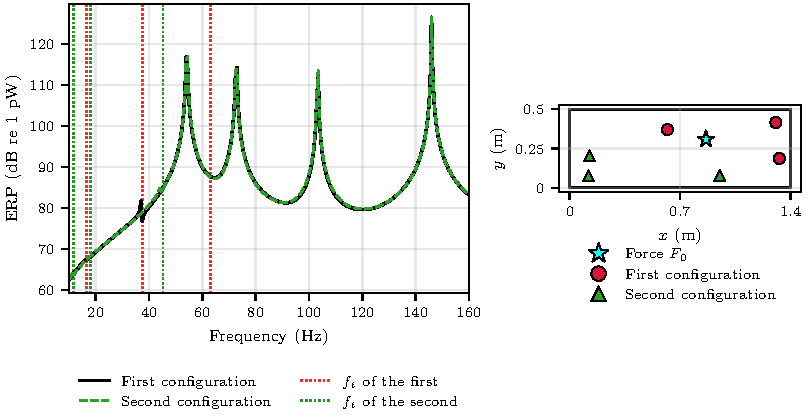
\includegraphics[max width=\textwidth]{Bilder/same_erp_different_resonators.pdf}
\caption[Two different designs with nearly the same ERP spectrum]{Two genuinely different three-resonator designs (different masses, positions and tuning frequencies) whose solver-computed ERP spectra are nearly identical (RMSE 0.39\,dB). Left: the two spectra overlaid, with the tuning frequencies of the resonators as dotted lines. Right: both resonator layouts on the plate, numbered by increasing tuning frequency.}
\label{fig:non-unique}
\end{figure}

\section{Uncertainty Quantification over Manufacturing Tolerances}

A design that looks good on paper is never built exactly as specified: a resonator's mass, position or tuning will always be off by a small amount once it is actually manufactured. Monte Carlo uncertainty quantification \parencite{metropolis1949monte} checks how much this matters. A chosen design is perturbed many times by small random amounts that match realistic manufacturing tolerances, for example a mass that is accurate to within two percent, and each perturbed version is evaluated with the fast forward surrogate. Collecting the resulting spectra gives a spread, instead of a single curve, which shows how sensitive a proposed design's acoustic behaviour is to the small errors that manufacturing will inevitably introduce. This only works with a fast surrogate model, since it needs many evaluations of the same design region, far more than the physics solver could provide in reasonable time.

\FloatBarrier
\newpage
\chapter{Research Concept}
\label{ch:concept}
\section{Design Space and Dataset}
\label{sec:design-space}

Every resonator in this thesis is described by five variables: its mass $m$, its tuning frequency $f_t$, its position $(x,y)$ on the plate, and a damping ratio $\zeta$. The stiffness is not sampled directly; it is derived from the mass and the tuning frequency, $k = m(2\pi f_t)^2$, so that the resonator is actually tuned to $f_t$ once it is placed on the plate. The damping coefficient is derived the same way, from the damping ratio, $c = 2\zeta\sqrt{km}$. All five variables are drawn together with Latin hypercube sampling \parencite{mckay1979lhs}, mass and tuning frequency and position uniformly, and the damping ratio on a logarithmic scale since it spans two orders of magnitude. The masses lie between 0.1 and 1.0\,kg, the tuning frequencies between 10 and 160\,Hz, the positions between 0.05\,m from the plate edges, and the damping ratios between $5\times10^{-4}$ and $8\times10^{-2}$; a point force of 1\,N acts at $(0.865, 0.309)$\,m. A configuration with several resonators simply repeats this for each one.

Sampling every variable directly like this matters more than it may first appear. Figure~\ref{fig:sampling-direct} shows the tuning-frequency distribution that Latin hypercube sampling of $f_t$ itself produces: it is close to uniform across the whole target band, as intended. Figure~\ref{fig:sampling-bias} shows what happens instead if only the mass and the stiffness are sampled directly and the tuning frequency is derived from them afterwards: the resulting tuning-frequency distribution is heavily skewed toward the low end of the band, even though mass and stiffness were each sampled evenly. The lesson from this comparison is that a dataset is only as balanced as the variables it samples directly; a quantity that is only derived from other sampled variables can end up badly distributed even if those other variables are not. This is why every physically meaningful design variable in this thesis, including the tuning frequency and the damping ratio, is sampled directly rather than derived.

\begin{figure}[h]
\centering
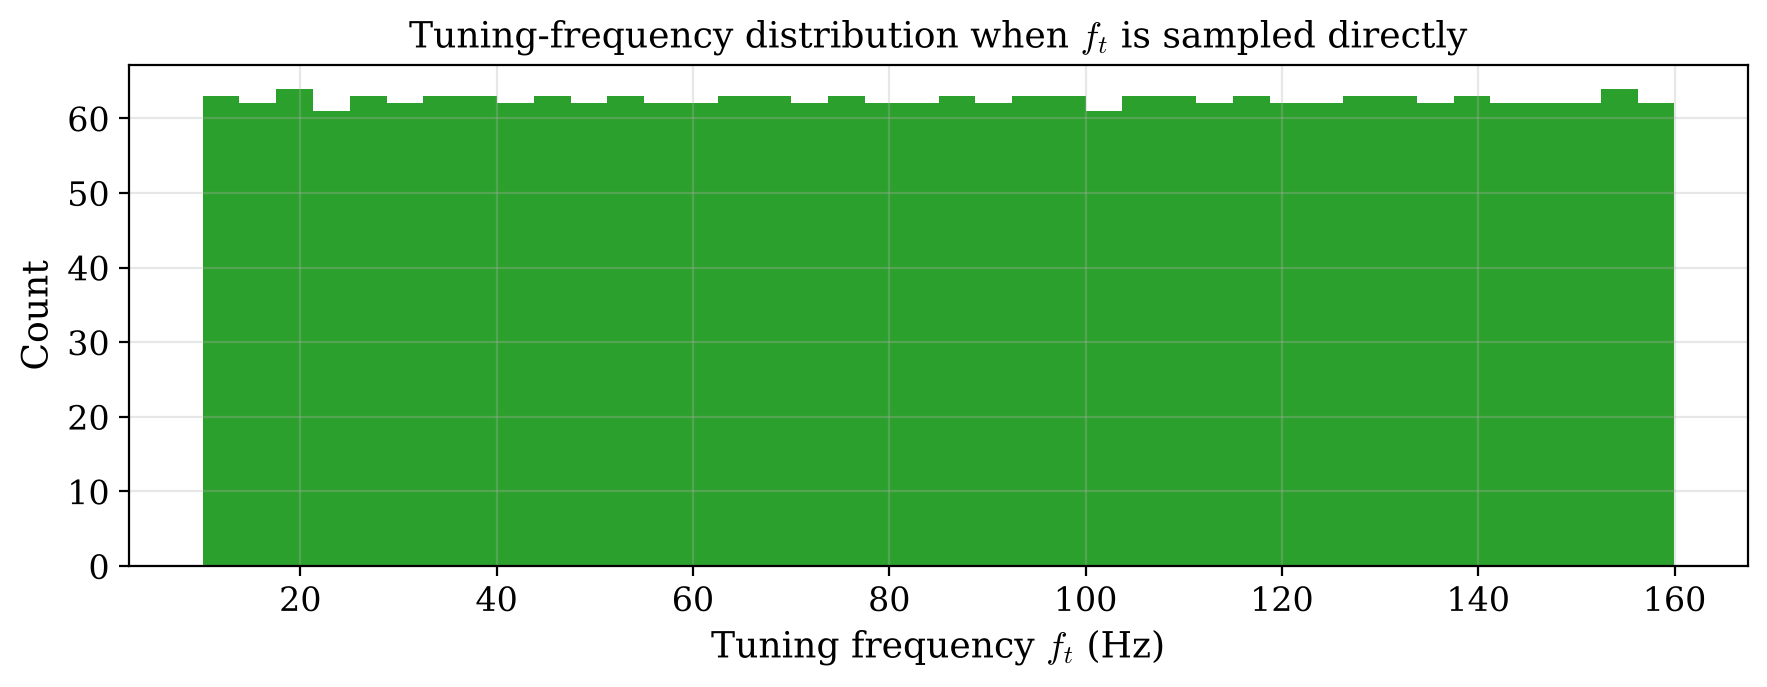
\includegraphics[width=0.95\textwidth]{Bilder/sampling_direct_ft.png}
\caption[Tuning frequency distribution when sampled directly]{Tuning-frequency distribution when $f_t$ is itself one of the sampled variables: close to uniform across the target band.}
\label{fig:sampling-direct}
\end{figure}

\begin{figure}[h]
\centering
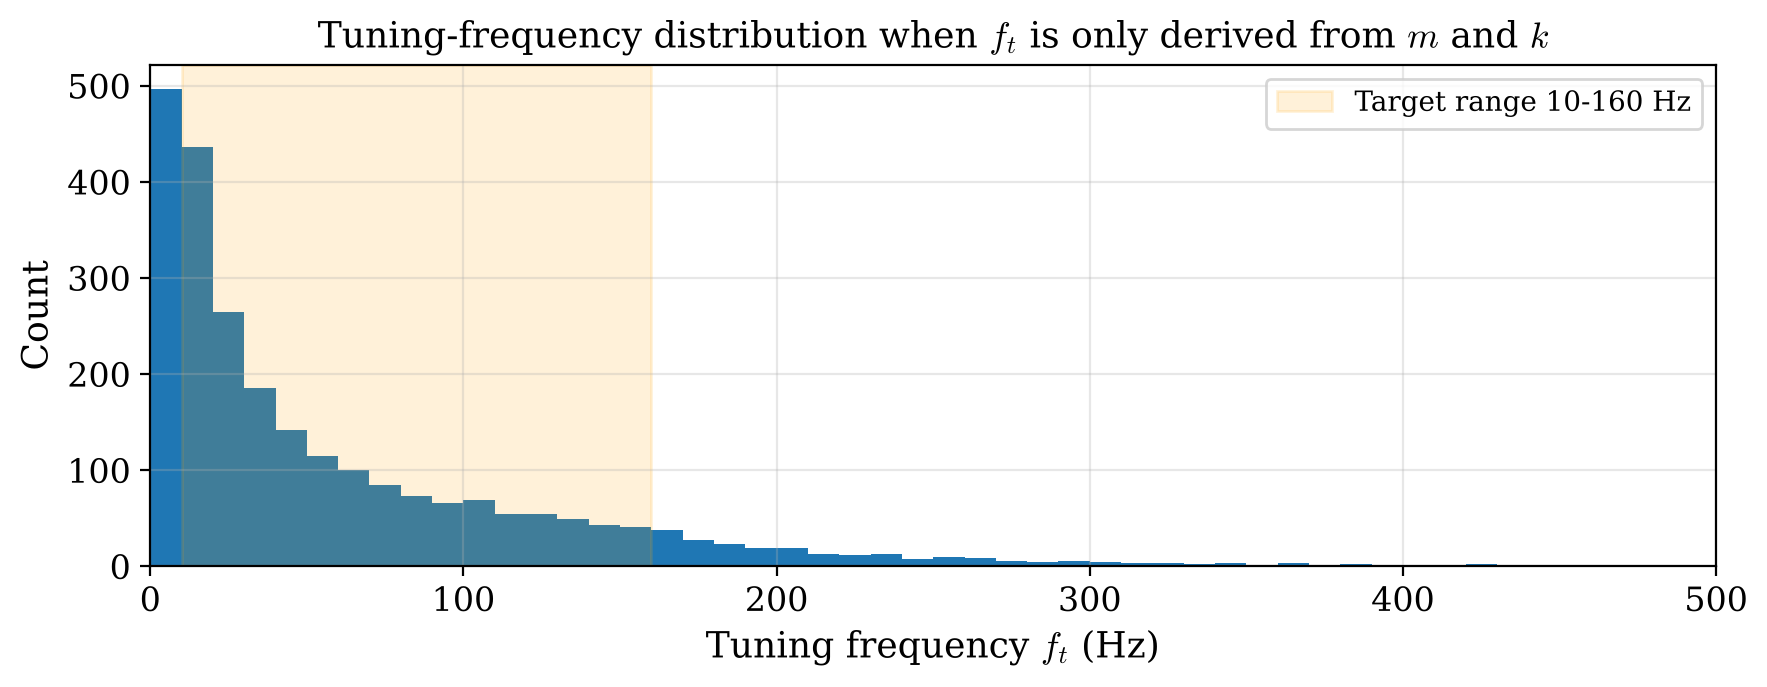
\includegraphics[width=0.95\textwidth]{Bilder/sampling_bias_mk.png}
\caption[Sampling bias when the tuning frequency is only derived]{Tuning-frequency distribution when mass and stiffness are sampled directly instead and the tuning frequency is only derived from them: the shaded target band is covered very unevenly.}
\label{fig:sampling-bias}
\end{figure}

For every sampled configuration, a modal physics solver computes the equivalent radiated power (ERP) spectrum at 301 frequencies between 10 and 160\,Hz. The plate's vibration is written as a sum of its own mode shapes plus the added resonator degrees of freedom, and the resulting linear system is solved at every frequency; the resonator degrees of freedom are then eliminated analytically so that only a small system, the size of the number of resonators, needs to be solved per frequency, which keeps dataset generation practical even for a hundred thousand configurations. Three datasets are used in this thesis, all solved with 18 plate modes ($6\times3$): two forward datasets of 100{,}000 configurations each, one with two and one with three resonators, in the five-variable design space described above, and an earlier two-resonator dataset of 200{,}000 configurations with four bounded design variables per resonator and a fixed damping coefficient, used for the invertible models (Section~\ref{sec:idon}). Figure~\ref{fig:erp-distribution} shows the resulting spread of ERP spectra across each of them, at every one of the 301 frequency points. The three datasets look alike: the ERP values average 84.0, 83.5 and 84.2\,dB with standard deviations of 9.8, 9.5 and 10.1\,dB, the median spectrum rises with frequency and shows clear peaks near the bare plate's own natural frequencies (dashed lines), and individual configurations vary widely around it, which is exactly the variety a surrogate model needs to learn from. The three-resonator dataset has a slightly lower mean and a smaller maximum than the two-resonator dataset, plausibly because a third resonator takes up more of the plate's vibration energy.

\begin{figure}[h]
\centering
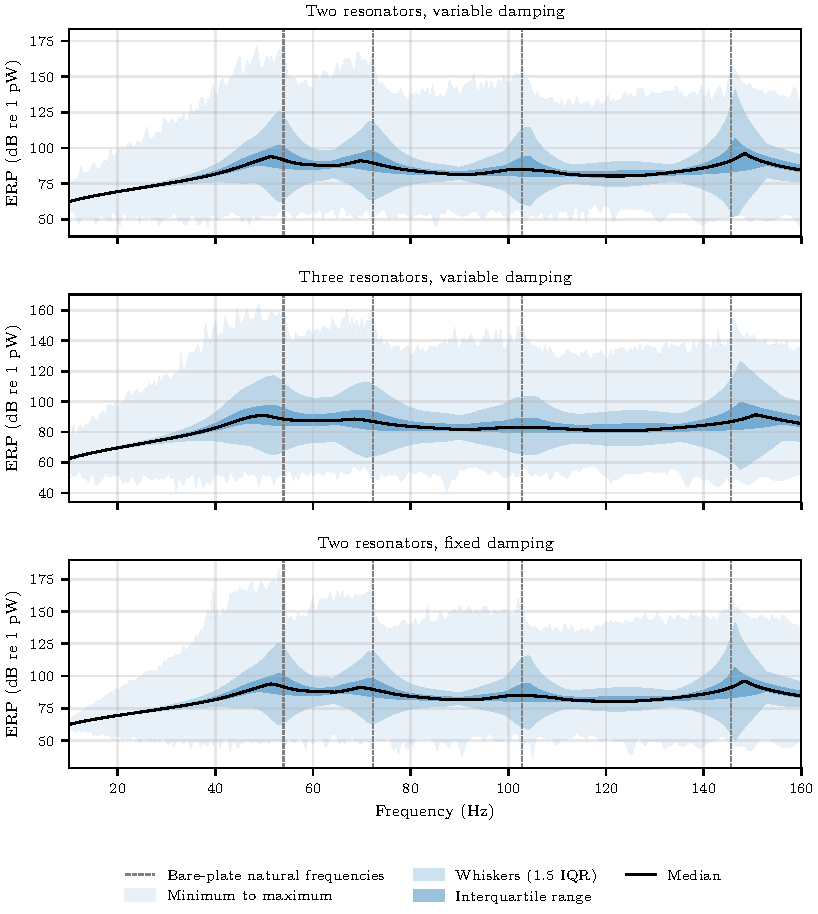
\includegraphics[max width=\textwidth]{Bilder/erp_distribution_datasets.pdf}
\caption[ERP distribution across the 301 frequency points]{Distribution of the ERP spectrum across all configurations of the three datasets, at each of the 301 frequency points: two resonators with sampled damping (100{,}000 configurations), three resonators with sampled damping (100{,}000) and two resonators with fixed damping (200{,}000). The shaded bands show the full range, the whiskers (1.5 times the interquartile range), the interquartile range and the median.}
\label{fig:erp-distribution}
\end{figure}

What does the biased sampling of Figure~\ref{fig:sampling-bias} actually do to the data a model would learn from? To check this directly, 2{,}000 configurations were sampled with mass and stiffness drawn directly and the tuning frequency derived, the same scheme as Figure~\ref{fig:sampling-bias}, and solved with the same solver. Figure~\ref{fig:erp-distribution-biased} shows the resulting ERP distribution, in the same style as the panels of Figure~\ref{fig:erp-distribution}. The overall spread of ERP values across this biased dataset is not noticeably smaller than the well-sampled one, but its median keeps sharp, tall peaks at the bare plate's natural frequencies (up to about 109\,dB, against about 96\,dB in the well-sampled dataset), because most resonators are tuned at low frequencies and hardly act on the plate's own resonances; what changes is where the data is concentrated. Because the derived tuning frequencies pile up at the low end of the band (Figure~\ref{fig:sampling-bias}), most of the training configurations are easy, repetitive examples from the same low-frequency region, while the higher part of the band is covered by only a handful of configurations. A model trained on this would see a low average test error, since most test examples fall in the dense, easy region it has seen many times, while being unreliable on the sparse, under-represented region. The average error alone would look good without the model having learned to generalise across the whole band; this is why this thesis reports accuracy at the resonance peaks separately from the overall accuracy, and why every design variable is sampled directly and evenly in the first place.

\begin{figure}[h]
\centering
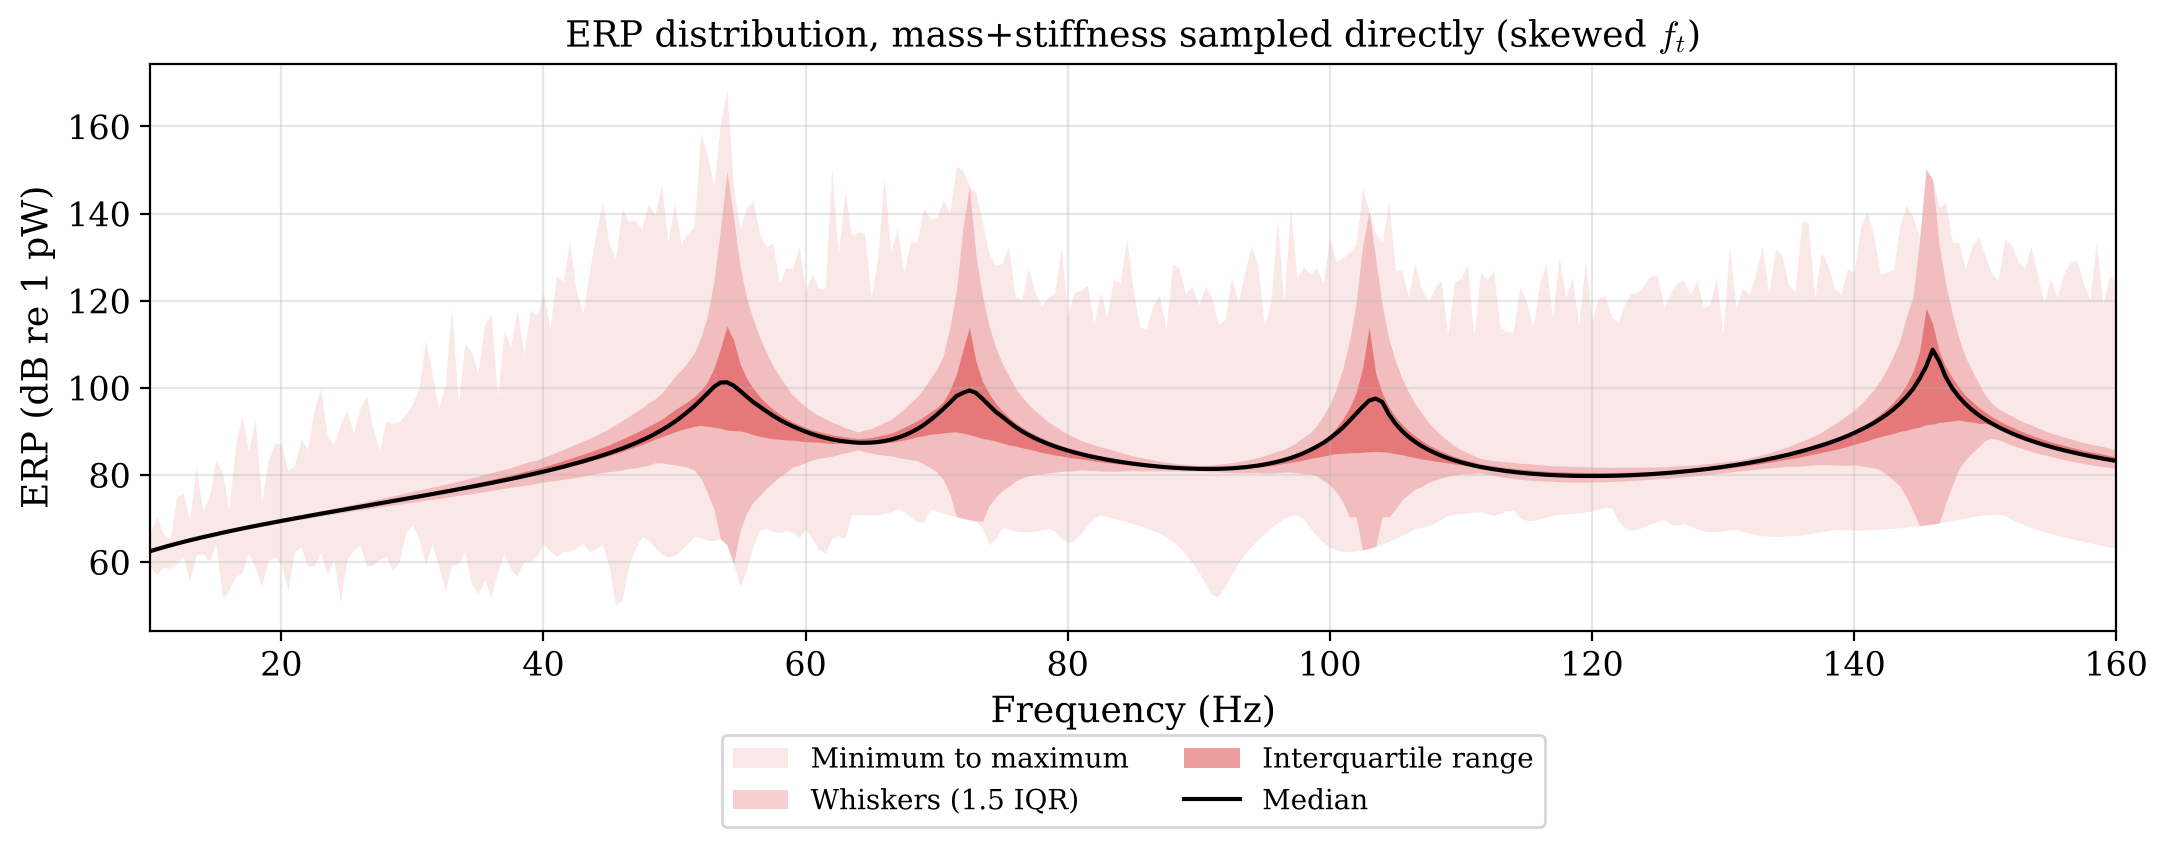
\includegraphics[width=0.95\textwidth]{Bilder/erp_distribution_biased.png}
\caption[ERP distribution under biased sampling]{ERP distribution of 2{,}000 configurations sampled the same way as Figure~\ref{fig:sampling-bias} (mass and stiffness sampled directly, tuning frequency derived and skewed low). Compare with Figure~\ref{fig:erp-distribution}.}
\label{fig:erp-distribution-biased}
\end{figure}

The dataset is split 80/10/10 into training, validation and test configurations, and every model in this thesis is trained and compared on the same split.

\section{Forward Architectures}
\label{sec:forward-architectures}

A forward architecture takes a resonator design and a query frequency as input and predicts the ERP value at that frequency. Nine of the ten architectures compared in this thesis share the same building blocks around a different core, shown in Figure~\ref{fig:forward-block}; only the plain baseline NN, described below, works on the raw design and frequency without them. The shared blocks are a resonator encoder that turns the set of resonators into a fixed-size description, since the plate's response does not depend on the order the resonators are listed in; a resonance query block that gives the network the distance between the query frequency and each resonator's tuning frequency; and a frequency encoder for the query frequency itself. The only part that changes between these architectures is the core architecture block; a shared decoder turns its output into the predicted ERP value.

\begin{figure}[h]
\centering
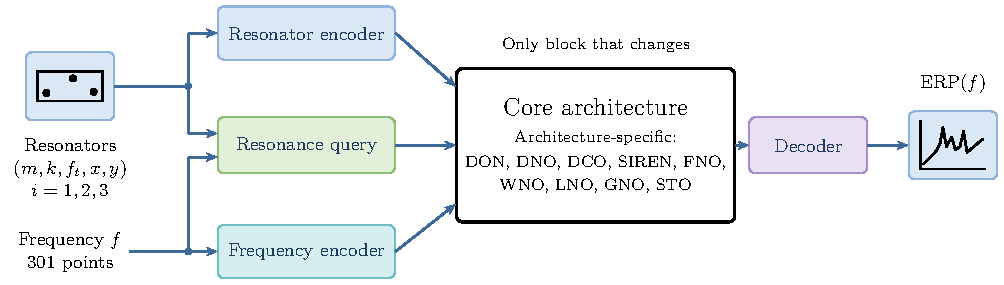
\includegraphics[max width=\textwidth]{Bilder/block_forward_architecture.pdf}
\caption[Forward architecture block diagram]{Shared structure of the nine encoder-based forward architectures: only the core architecture block changes between them. The baseline NN has no encoder blocks.}
\label{fig:forward-block}
\end{figure}

The ten forward architectures are, in short:

\begin{itemize}
  \item \textbf{DON} (DeepONet): a branch network encodes the design, a trunk network encodes the frequency, and the two are combined into a spectrum through a shared, orthonormal frequency basis \parencite{lu2021deeponet}.
  \item \textbf{DNO} and \textbf{DCO}: two architectures developed for this thesis rather than taken from a specific paper, which build on a stack of residual blocks \parencite{he2016resnet} in two different ways: DNO modulates each block with the resonator encoding through feature-wise linear modulation \parencite{perez2018film}, DCO concatenates the encodings of the resonators and of the frequency before the blocks.
  \item \textbf{SIREN}: a network of sine-activated layers, which tends to fit smooth oscillatory signals well \parencite{sitzmann2020siren}.
  \item \textbf{FNO} (Fourier neural operator): processes the frequency axis with learned convolutions in the Fourier domain \parencite{li2021fno}.
  \item \textbf{WNO} (wavelet neural operator): the same idea with a wavelet transform instead, which can better localise sharp resonance peaks \parencite{tripura2022wno}.
  \item \textbf{LNO} (Laplace neural operator): represents the spectrum through a small set of learned poles and residues, a natural fit for a system built from resonances \parencite{cao2023lno}.
  \item \textbf{GNO} (graph neural operator): treats the resonators as nodes of a graph and lets them exchange messages before predicting the spectrum \parencite{li2020graphno,gilmer2017mpnn}.
  \item \textbf{STO} (Set Transformer operator): uses attention between the resonators and the query frequency instead of message passing \parencite{lee2019settransformer,vaswani2017attention}.
  \item \textbf{NN}: a plain feed-forward network on the raw design and frequency (a multilayer perceptron, a universal approximator of continuous functions \parencite{hornik1989approximation}), used as a simple baseline.
\end{itemize}

Every architecture is sized to about 145{,}000 parameters (between 143{,}000 and 156{,}000 for the two forward datasets), so that differences in accuracy reflect the architecture itself rather than one model simply being larger than another.

\section{Invertible Architectures and Generative Design}

An invertible architecture is built the same way as a forward one, except that its core is made of blocks that can be run backward as well as forward. Running it forward predicts a spectrum from a design, exactly like the forward architectures above; running the same weights backward turns a target spectrum into a proposed design. Figure~\ref{fig:operators-overview} summarises the difference between the three kinds of model used in this thesis: a forward operator maps one design to one spectrum; an inverse-only operator would map one spectrum to many possible designs; an invertible operator does both with the same weights, so the two directions stay consistent with each other.

\begin{figure}[h]
\centering
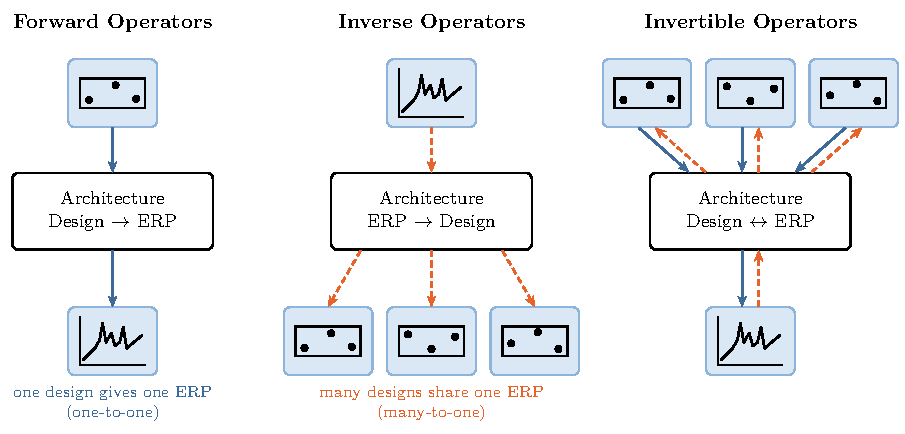
\includegraphics[max width=\textwidth]{Bilder/block_operators_overview.pdf}
\caption[Forward, inverse and invertible operators]{Forward operators map one design to one spectrum (one-to-one); the inverse direction maps one spectrum to many possible designs (many-to-one); an invertible operator combines both directions in one set of weights.}
\label{fig:operators-overview}
\end{figure}

This two-direction property is what makes generative design possible: given a target ERP spectrum, for example one with a deep notch at a frequency an engineer wants quiet, the inverse direction proposes one or several resonator designs that should produce it, without needing a separate search or optimisation loop. A proposed design can then be checked by running it back through the forward direction, or through the physics solver directly, and its robustness to manufacturing tolerances can be checked with the Monte Carlo procedure described in Chapter~\ref{ch:theory}. This thesis builds seven invertible architectures: an invertible DeepONet (iDON), described in Section~\ref{sec:idon}, and an iFNO family of six more architectures, described in Section~\ref{sec:ifno}.

\subsection{iDON}
\label{sec:idon}

iDON \parencite{kaltenbach2023invertible} keeps the DeepONet idea of a branch network for the design and a trunk network for the frequency, but makes the branch itself exactly invertible, shown in Figure~\ref{fig:idon-block}. The branch is a RealNVP coupling flow \parencite{dinh2017realnvp}: it maps the design $a$ to a vector of $Q$ coefficients $b$, and because every RealNVP layer is a coupling block of the kind described in Chapter~\ref{ch:theory}, this map can be run backward to recover $a$ from $b$ exactly, with no approximation. The trunk is an ordinary network that maps the frequency to an orthonormal basis $\Psi(f)$, shared by both directions. In this thesis the branch consists of ten RealNVP coupling layers with 256 hidden units each, and the trunk applies four hidden layers of 256 units to the frequency and to its sine and cosine features at 32 harmonics. The forward direction predicts the spectrum as $\mathrm{ERP}(f) = \Psi(f)\,b + \psi_0$; the inverse direction projects a target spectrum onto the same basis, $b^\ast = \Psi^T(y - \psi_0)/F$, and runs the branch backward to recover a design from $b^\ast$.

\begin{figure}[h]
\centering
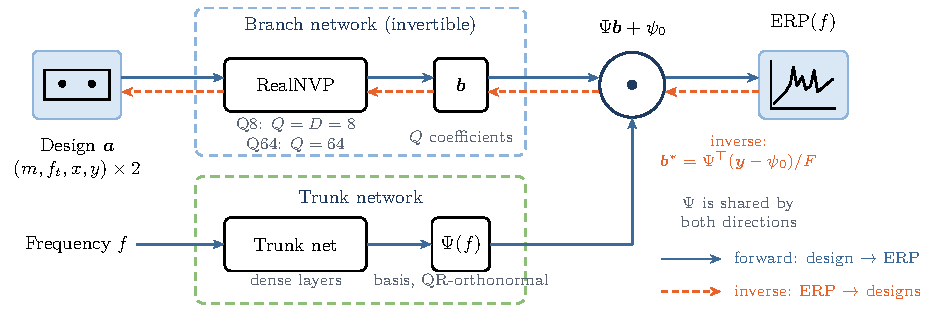
\includegraphics[max width=\textwidth]{Bilder/block_idon_architecture.pdf}
\caption[iDON block diagram]{iDON: an invertible RealNVP branch network maps a design to $Q$ coefficients and back; an ordinary trunk network supplies a shared, orthonormal frequency basis.}
\label{fig:idon-block}
\end{figure}

The numbers reported for iDON and the iFNO family in this section and in Chapter~\ref{ch:results} come from an earlier, larger two-resonator dataset of 200{,}000 configurations, built before the damping ratio became a sampled design variable: each resonator is described by four bounded numbers, mass, tuning frequency and position, with a fixed damping coefficient. The architectures and the invertibility mechanism are identical to the ones described here; only this particular dataset predates the five-variable design space of Section~\ref{sec:design-space}.

How many coefficients $Q$ should the branch produce? The most direct choice is $Q = D$, the number of numbers in the design itself (so a two-resonator design with four bounded numbers each gives $D=8$); this thesis calls that configuration Q8. A strictly invertible branch with $Q=D$ is bijective, but it also means the basis $\Psi(f)$ has only as many degrees of freedom as the design, which turned out to be too few to represent the ERP spectrum well: on the two-resonator, 200{,}000-configuration dataset used for the invertible models, Q8 reaches only 6.05\,dB forward RMSE and recovers the tuning frequency with a Pearson correlation of 0.81 (Table~\ref{tab:idon-q}). The fix used in this thesis, and in \textcite{kaltenbach2023invertible}, is to pad the branch to a larger $Q$, for example $Q=64$ (Q64): the branch still outputs a vector of length $Q$, but only the first $D$ numbers correspond to the physical design, and the remaining $Q-D$ are extra, padded latent values $z$ that have no physical meaning. With more coefficients to work with, the trunk can represent the spectrum far more accurately: Q64 reaches 2.67\,dB forward RMSE, and recovers the tuning frequency with a Pearson correlation of 0.87, a clear improvement over Q8 on every metric checked in this thesis. The padding only helps if the extra latent values stay small and uninformative, otherwise the model could hide part of the true design signal in them where the inverse direction cannot see it; this is enforced by adding a padding loss term, $\mathcal L_\text{pad} = \mathrm{Huber}(\hat z, 0)$ \parencite{huber1964robust}, that pulls the recovered padded values toward zero during training. Every result for iDON reported in Chapter~\ref{ch:results} uses the padded Q64 configuration.

\subsection{iFNO and the Rest of the Family}
\label{sec:ifno}

The other six invertible architectures, iDNO, iDCO, iFNO, iLNO, iGNO and iSTO, share one common pipeline instead of each being built from scratch, shown in Figure~\ref{fig:ifno-block}. A design is lifted to a latent representation by a block $P$, together with the query frequency; the latent representation passes through a coupling stack, the same kind of invertible block described in Chapter~\ref{ch:theory}, which uses the same weights in both directions; a readout block $Q$ turns the latent representation into the predicted ERP. The inverse direction mirrors this exactly: a lift $P'$ turns a target spectrum into a latent representation, the same coupling stack runs backward, and a readout $Q'$ turns the result into a proposed design.

\begin{figure}[h]
\centering
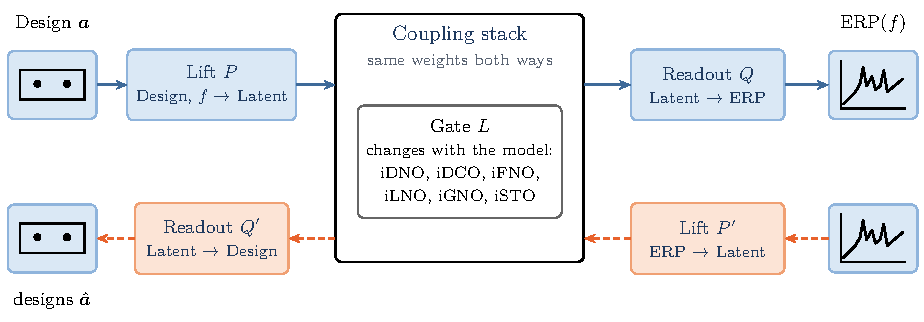
\includegraphics[max width=\textwidth]{Bilder/block_invertible_operator_architecture.pdf}
\caption[iFNO family block diagram]{Shared pipeline of the iFNO family. Only the gate $L$ inside the coupling stack changes between iDNO, iDCO, iFNO, iLNO, iGNO and iSTO; the lifts, readouts and the rest of the coupling stack are the same.}
\label{fig:ifno-block}
\end{figure}

Only the coupling stack is an exact bijection between latent tensors; the lifts and readouts are ordinary, learned (and therefore lossy) networks, so the pipeline as a whole is a bidirectional model with an invertible core rather than an exactly invertible map from design to spectrum. What distinguishes the six family members from one another is only the gate $L$ inside each coupling block: iDNO uses a residual-block gate conditioned on a learned embedding of the frequency, matching DNO \parencite{perez2018film}; iDCO uses a residual-block gate matching DCO \parencite{he2016resnet}; iFNO uses a spectral convolution gate, the invertible counterpart of the FNO core \parencite{li2021fno}; iLNO uses a learned pole-residue gate matching LNO \parencite{cao2023lno}; iGNO uses a graph message-passing gate matching GNO \parencite{li2020graphno}; and iSTO uses a frequency-mixing gate in place of STO's attention \parencite{lee2019settransformer}. This mirrors how the nine encoder-based forward architectures in Section~\ref{sec:forward-architectures} share an encoder and a decoder and differ only in their core block: here, the lift, coupling stack and readout stay fixed, and only the gate inside the coupling stack is architecture-specific. Training follows the three-stage recipe of \textcite{long2025invertiblefno}, detailed in Section~\ref{sec:training}: first the invertible core and the lifts and readouts, then a $\beta$-variational step \parencite{kingma2014vae,higgins2017betavae} that turns a single estimated design into a small family of plausible designs (needed because, as Chapter~\ref{ch:theory} showed, the inverse is rarely unique), then all parts trained together.

\section{Training}
\label{sec:training}

All models are trained on the 80/10/10 split described in Section~\ref{sec:design-space}, with the ERP and the design variables normalised by the statistics of the training split, and the weights of the epoch with the lowest validation loss are kept.

The ten forward architectures are trained for 200 epochs with a batch size of 128 using AdamW \parencite{loshchilov2019adamw} with a weight decay of $10^{-4}$, a learning rate of $5\times10^{-4}$ ($2\times10^{-4}$ for SIREN) that decays along a cosine schedule to $10^{-6}$, and gradient-norm clipping at 5. The loss is not the plain mean squared error. It adds the mean squared error of the spectrum's slope between neighbouring frequencies, with weight 0.5, and the squared error at the resonance peaks of the target spectrum, with weight 0.05, so that the narrow peaks, which carry most of the acoustic information, are not neglected. NN has no permutation-invariant encoder, so the order of the resonators is shuffled in every batch to keep it from depending on the order.

The six architectures of the iFNO family are trained in three stages, as described in Section~\ref{sec:ifno}, with up to 100, 25 and 50 epochs, learning rates of $5\times10^{-4}$, $10^{-3}$ and $3\times10^{-4}$ with a cosine decay, a batch size of 128 and gradient-norm clipping at 5. The weight of the variational term is $\beta = 0.05$, reached after a warm-up over the first 8 epochs of the second stage \parencite{higgins2017betavae}, and the cycle-consistency and alignment terms of the first and third stage have weight 0.1. A stage ends early if its validation loss has not improved for 10 epochs. This happened in the first stage of iFNO (after 65 epochs) and iGNO (71 epochs) and in the third stage of iFNO (after 25 epochs); iLNO and iSTO ran the full 100, 25 and 50 epochs. iDNO and iDCO were trained with a shorter schedule of 50, 15 and 15 epochs, so their results in Chapter~\ref{ch:results} may improve with the full schedule.

iDON is trained for 150 epochs with a learning rate of $5\times10^{-4}$. Its loss is the sum of the forward spectrum loss above, whose peak term is only switched on in the last 20\,\% of the epochs, a Huber loss \parencite{huber1964robust} on the design recovered from the true spectrum, whose weight rises from zero to one over the first 10 epochs, and the padding term of Section~\ref{sec:idon} with weight 0.1. The Q8 variant stopped early: its validation loss stopped improving after epoch 37, and training ended after 50 of the 150 planned epochs, whereas Q64 ran all 150 epochs.

The invertible operators were not all trained with the same parameters and epochs: the training was carried out on a CPU, with only limited GPU session time available, so the learning rates, the number of epochs and the stage schedules were chosen to fit the available compute and differ between models, as described above. Results from further training runs with other settings, if they become available, will be published in the GitHub repository (and the LRZ Sync\&Share folder) given in Appendix~B.

\section{A Single, Reproducible Pipeline}

The physics solver, the dataset generation, the ten forward architectures and the seven invertible architectures described above are all implemented in one Python script. Running it solves resonator configurations, builds a dataset, and trains and evaluates whichever models are selected, without any other setup. This was a deliberate choice: keeping the whole pipeline in one place, with one consistent way of encoding a design and one consistent training loop, makes the results in this thesis straightforward for another person to reproduce from the dataset variables and architecture descriptions given above.

\FloatBarrier
\newpage

\chapter{Results}
\label{ch:results}
\section{Forward Surrogates: Two Resonators}

All ten forward architectures are trained on the same dataset, 100{,}000 configurations of two resonators each, for 200 epochs, and compared on the same 10{,}000-configuration test split. Table~\ref{tab:forward-results} reports the root-mean-square error (RMSE) between each model's predicted ERP spectrum and the solver's, the coefficient of determination ($R^2$), the Pearson correlation, and the RMSE restricted to the resonance peaks, which is usually the hardest part of the spectrum to get right. The architectures are listed in the same order throughout this chapter, with the plain feed-forward baseline NN last.

\begin{table}[h]
\centering
\caption[Forward surrogate comparison on the test split]{Forward architectures on the two-resonator test split (10{,}000 spectra). Lower RMSE and higher $R^2$ and Pearson $r$ are better.}
\label{tab:forward-results}
\begin{tabular}{lrrrrr}
\hline
Model & Parameters & RMSE (dB) & $R^2$ & Pearson $r$ & RMSE at peaks (dB) \\
\hline
DON   & 144{,}756 & 3.939 & 0.8369 & 0.9405 & 7.151 \\
DNO   & 143{,}434 & 1.212 & 0.9846 & 0.9924 & 3.841 \\
DCO   & 147{,}094 & 1.113 & 0.9870 & 0.9936 & 3.706 \\
SIREN & 145{,}820 & 1.538 & 0.9752 & 0.9879 & 4.315 \\
FNO   & 145{,}050 & 1.834 & 0.9646 & 0.9841 & 5.278 \\
WNO   & 146{,}318 & 1.956 & 0.9598 & 0.9818 & 6.557 \\
LNO   & 144{,}199 & 1.430 & 0.9785 & 0.9896 & 4.230 \\
GNO   & 143{,}718 & 2.107 & 0.9533 & 0.9805 & 4.801 \\
STO   & 144{,}213 & 2.096 & 0.9538 & 0.9799 & 4.894 \\
NN    & 144{,}481 & 6.241 & 0.5907 & 0.8417 & 11.747 \\
\hline
\end{tabular}
\end{table}

DCO and DNO, the two architectures developed specifically for this thesis, come out ahead of the others, with DCO reaching about 1.1\,dB RMSE on unseen designs. LNO and SIREN follow, FNO, WNO, STO and GNO lie between 1.8 and 2.1\,dB, and DON reaches 3.9\,dB. The plain feed-forward baseline, NN, is clearly the weakest, which confirms that giving the network an explicit, permutation-invariant encoder for the resonator set and physics-aware frequency features, which every other architecture uses and NN does not, is worth the added complexity.

The averages hide how the errors are distributed over the test split. Computed per spectrum, the median RMSE of DCO is only 0.82\,dB, and for every architecture except DON and NN at most 0.5\,\% of the test spectra have an RMSE above 5\,dB (13.8\,\% for DON and 88.4\,\% for NN). Figure~\ref{fig:forward-best-2res} shows, for each architecture, the test spectrum it predicts best. Every architecture except NN reproduces the solver curve almost exactly, with an RMSE between 0.2 and 1.2\,dB (3.6\,dB for NN). In most of these cases (seven of the ten) at least one resonator is tuned below the first plate resonance at about 54\,Hz, where it hardly changes the response, so the spectrum stays close to that of the bare plate and is easy to learn. Figure~\ref{fig:forward-worst-2res} shows the opposite end, the test spectrum each architecture predicts worst. The errors there range from 5.4\,dB (WNO) to 9.4\,dB (DON), and 11.8\,dB for NN, and they arise in the same place: the two resonators are tuned in the upper part of the band, mostly above 120\,Hz and often within a few hertz of each other, where the resonance peaks are narrow and overlap, so the predictions smooth them out or place them at slightly wrong frequencies. In most of these worst cases one resonator also sits close to the force position, where it couples most strongly to the plate. Even then, the first plate resonances at lower frequencies are reproduced well by every architecture except NN.

\begin{figure}[p]
\centering
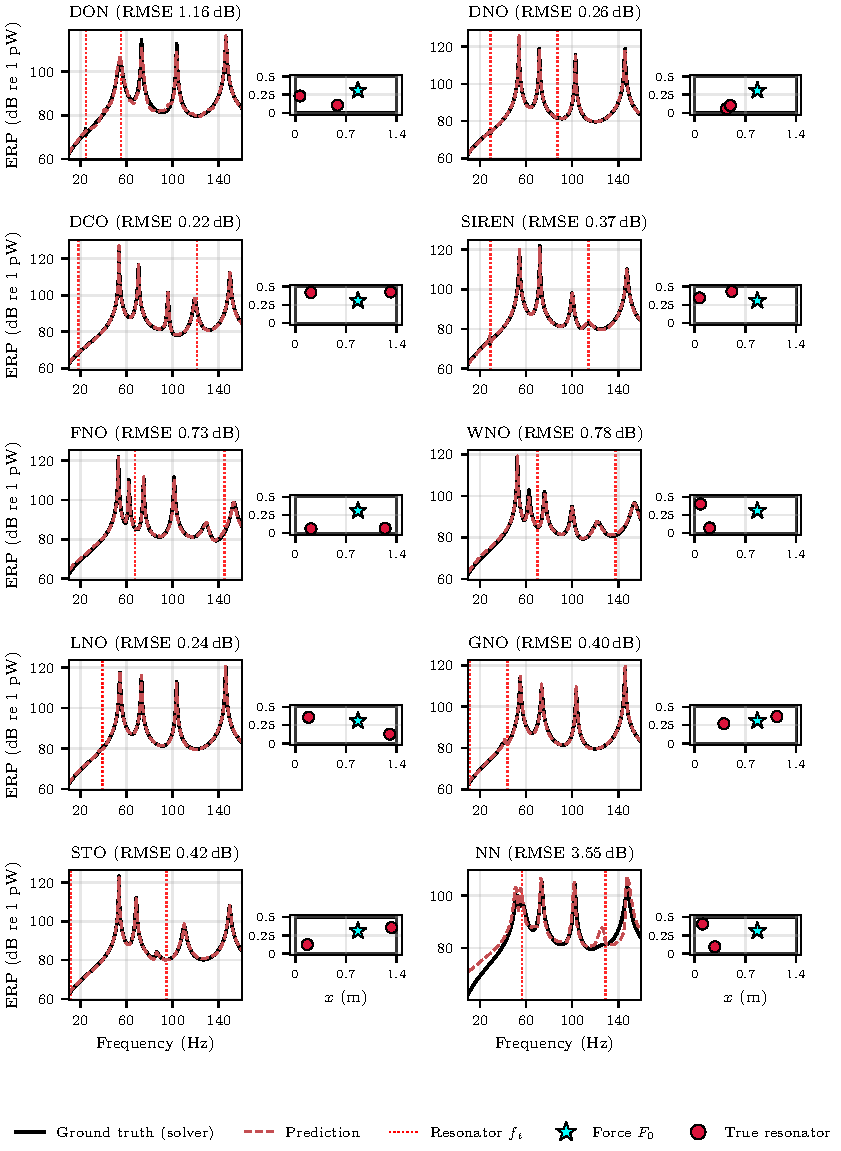
\includegraphics[max width=\textwidth,max height=0.84\textheight]{Bilder/forward_models_best_case_two_resonators.pdf}
\caption[Best test spectrum of each forward architecture, two resonators]{Best case of each forward architecture on the two-resonator test split: the test spectrum with the lowest RMSE, solver (black) against prediction (red dashed), with the resonator layout of that spectrum on the plate next to it.}
\label{fig:forward-best-2res}
\end{figure}

\begin{figure}[p]
\centering
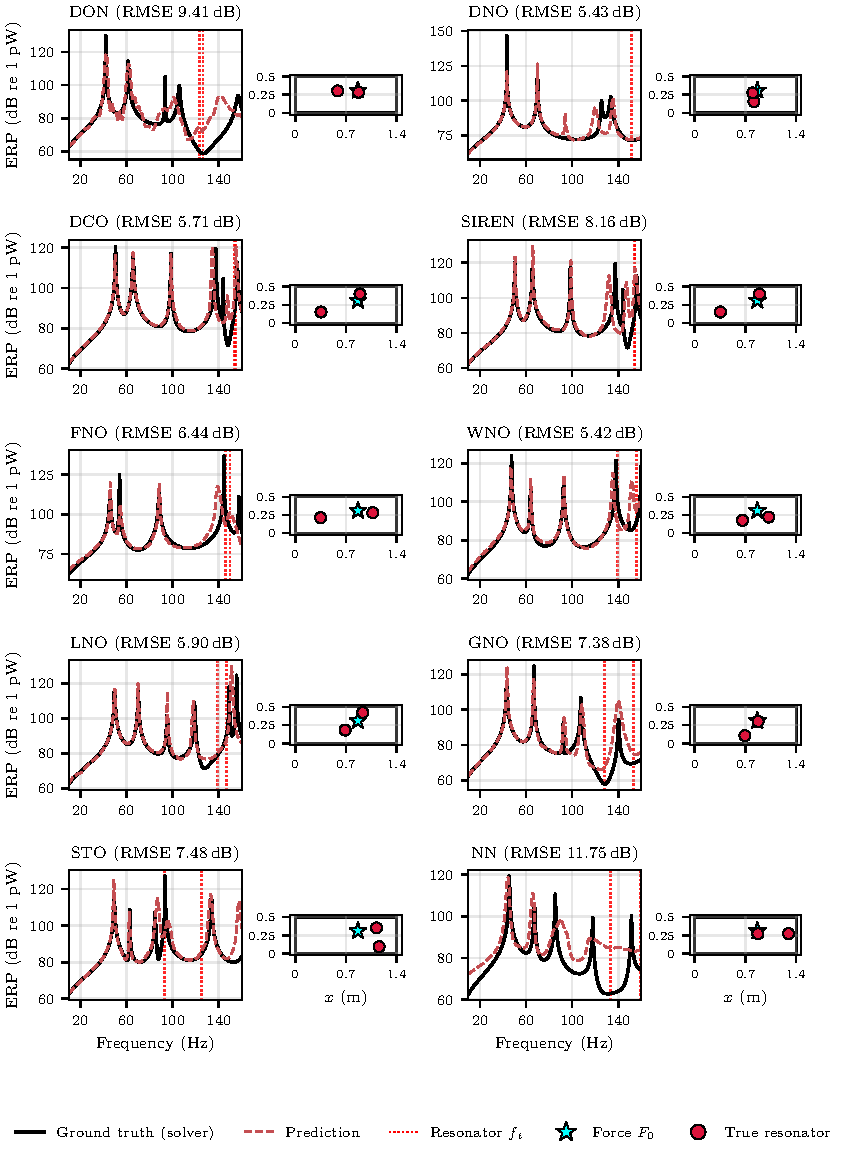
\includegraphics[max width=\textwidth,max height=0.84\textheight]{Bilder/forward_models_worst_case_two_resonators.pdf}
\caption[Worst test spectrum of each forward architecture, two resonators]{Worst case of each forward architecture on the two-resonator test split: the test spectrum with the highest RMSE. The largest disagreements occur at resonances in the upper part of the band, where the two tuned resonators lie close together.}
\label{fig:forward-worst-2res}
\end{figure}

Figure~\ref{fig:dco-parity} (left) shows DCO's predictions against the solver's values across the whole two-resonator test split: the points follow the ideal line closely over the whole range of ERP values ($R^2 = 0.987$), with the spread growing at the highest ERP values, which occur at the resonance peaks.

\begin{figure}[h]
\centering
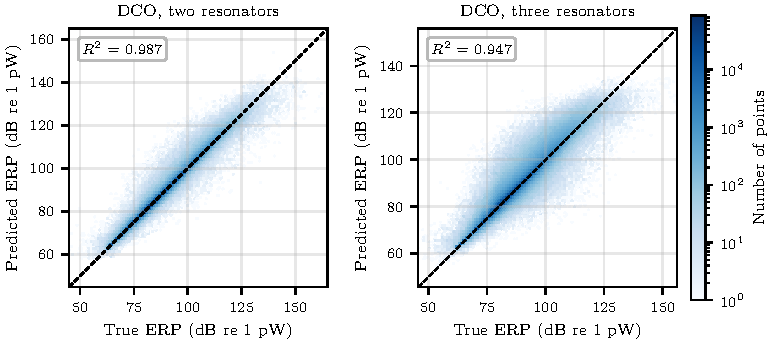
\includegraphics[max width=\textwidth]{Bilder/forward_dco_prediction_vs_true_erp.pdf}
\caption[DCO predicted versus true ERP]{DCO: predicted ERP against the solver's ERP, across the full test split of the two-resonator (left) and the three-resonator (right) dataset. Colour shows the number of points per cell on a logarithmic scale.}
\label{fig:dco-parity}
\end{figure}

\section{Forward Surrogates: Three Resonators}
\label{sec:results-3res}

The same ten architectures are also compared on a three-resonator dataset of 100{,}000 configurations. It is generated exactly like the two-resonator dataset: the same plate, the same 18 plate modes ($6\times3$), and the same five-variable design space with a sampled damping ratio; only the number of resonators per configuration changes. Table~\ref{tab:forward-results-3res} reports the same metrics as Table~\ref{tab:forward-results}.

\begin{table}[h]
\centering
\caption[Forward surrogate comparison, three resonators]{Forward architectures on the three-resonator test split (10{,}000 spectra, 18 plate modes).}
\label{tab:forward-results-3res}
\begin{tabular}{lrrrrr}
\hline
Model & Parameters & RMSE (dB) & $R^2$ & Pearson $r$ & RMSE at peaks (dB) \\
\hline
DON   & 151{,}560 & 4.677 & 0.7593 & 0.9104 & 8.139 \\
DNO   & 150{,}238 & 2.271 & 0.9432 & 0.9735 & 5.252 \\
DCO   & 155{,}536 & 2.186 & 0.9474 & 0.9753 & 5.238 \\
SIREN & 153{,}002 & 2.481 & 0.9322 & 0.9690 & 5.516 \\
FNO   & 153{,}870 & 2.773 & 0.9153 & 0.9594 & 6.510 \\
WNO   & 153{,}626 & 3.046 & 0.8979 & 0.9530 & 7.324 \\
LNO   & 152{,}011 & 2.688 & 0.9205 & 0.9642 & 5.781 \\
GNO   & 143{,}718 & 2.659 & 0.9222 & 0.9690 & 4.874 \\
STO   & 144{,}213 & 2.930 & 0.9055 & 0.9626 & 5.308 \\
NN    & 145{,}489 & 7.159 & 0.4358 & 0.7980 & 12.581 \\
\hline
\end{tabular}
\end{table}

The top and the bottom of the ranking are the same as in the two-resonator case: DCO and DNO still lead, with 2.19\,dB and 2.27\,dB, and NN and DON are still the weakest. In the middle the order changes: SIREN stays close behind the two leaders, GNO moves from eighth to fourth place, and with 4.87\,dB it now has the lowest RMSE at the resonance peaks of all ten architectures, although its overall RMSE is only middling. What changes most is the overall difficulty: the RMSE of the best architectures roughly doubles going from two to three resonators (DCO from 1.11\,dB to 2.19\,dB, DNO from 1.21\,dB to 2.27\,dB, LNO from 1.43\,dB to 2.69\,dB), while the weaker architectures increase less (DON from 3.94\,dB to 4.68\,dB, NN from 6.24\,dB to 7.16\,dB). Overall the increase is a factor of 1.1 to 2.0. With a third resonator there are more mode shapes to couple to, more possible near-coincidences between tuning frequencies, and a higher-dimensional design to encode, so this increase is expected. That the best and the worst architectures stay the same under a harder problem is evidence that the comparison in Table~\ref{tab:forward-results} reflects a real property of each architecture, not an artefact of the easier two-resonator case. The right panel of Figure~\ref{fig:dco-parity} shows the same effect for DCO: the $R^2$ drops from 0.987 to 0.947 and the cloud around the ideal line widens.

Figure~\ref{fig:forward-best-3res} and Figure~\ref{fig:forward-worst-3res} show the best and the worst test spectrum of every architecture, as for two resonators. In the best cases every architecture except NN is within 1.4\,dB of the solver (NN: 3.6\,dB), and every one of these configurations has at least one resonator tuned below the first plate resonance. The worst cases reach 8.3 to 11.6\,dB (12.7\,dB for NN), again with resonators tuned in the upper half of the band, and they are largely shared between architectures: SIREN, FNO, GNO and STO all fail most on the same configuration (tuning frequencies of about 106, 148 and 154\,Hz), DNO and WNO fail most on another one (131, 140 and 151\,Hz), and DON and NN on a third. A configuration that is hard for one architecture is therefore usually hard for the others as well, which points to the physics of closely spaced, strongly coupled resonances rather than to a weakness of any single architecture. Only 1.6 to 4.2\,\% of the test spectra of DNO, DCO, SIREN, FNO, WNO, LNO, GNO and STO have an RMSE above 5\,dB, against 31.8\,\% for DON and 98.7\,\% for NN.

\begin{figure}[p]
\centering
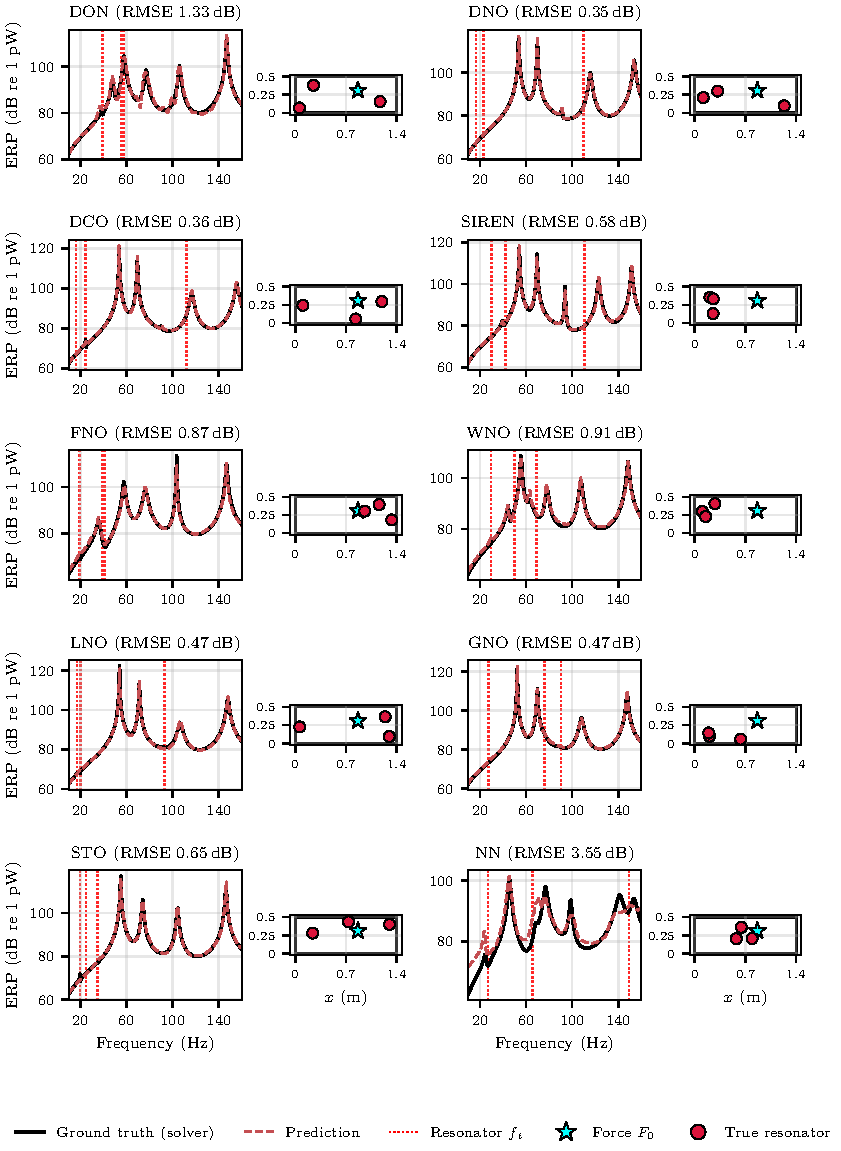
\includegraphics[max width=\textwidth,max height=0.84\textheight]{Bilder/forward_models_best_case_three_resonators.pdf}
\caption[Best test spectrum of each forward architecture, three resonators]{Best case of each forward architecture on the three-resonator test split, in the same format as Figure~\ref{fig:forward-best-2res}.}
\label{fig:forward-best-3res}
\end{figure}

\begin{figure}[p]
\centering
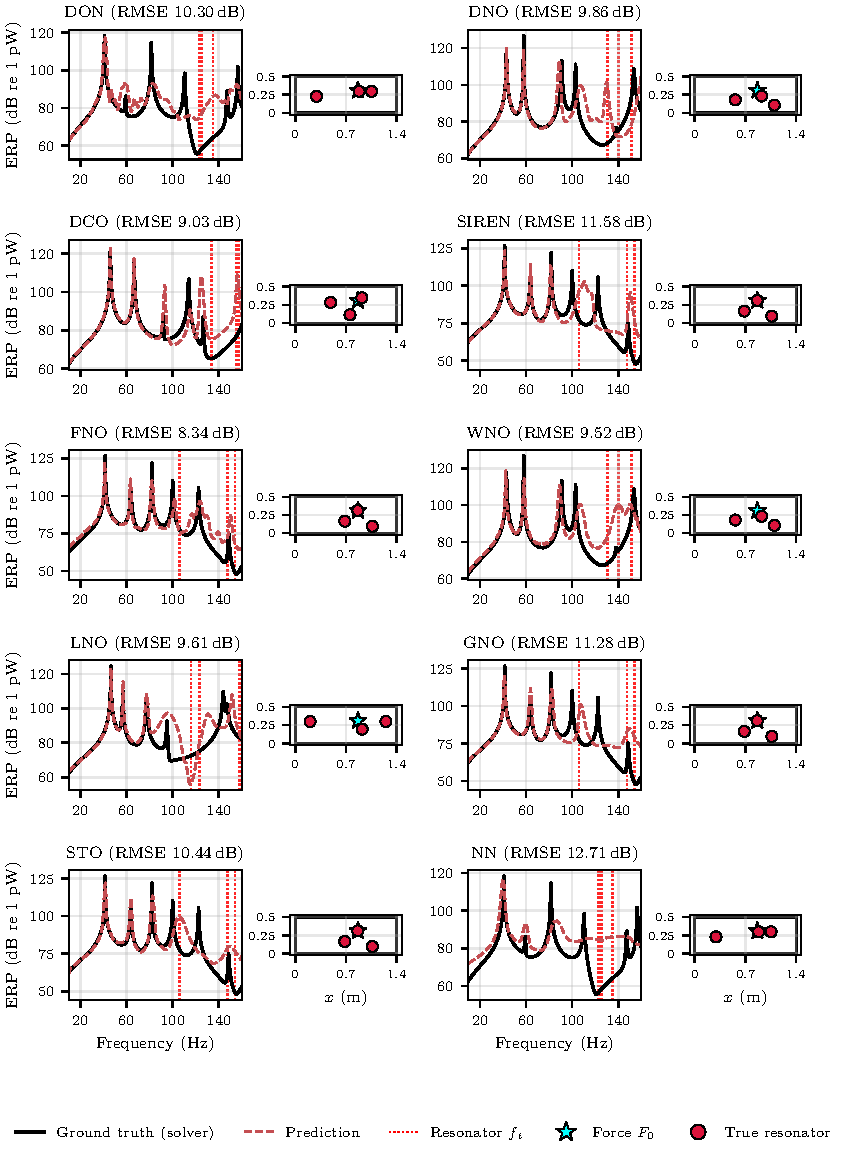
\includegraphics[max width=\textwidth,max height=0.84\textheight]{Bilder/forward_models_worst_case_three_resonators.pdf}
\caption[Worst test spectrum of each forward architecture, three resonators]{Worst case of each forward architecture on the three-resonator test split. Several architectures fail on the same configurations, where resonators are tuned in the upper part of the band.}
\label{fig:forward-worst-3res}
\end{figure}

\section{Invertible Operators and Generative Design}

The invertible architectures described in Section~\ref{sec:idon} and Section~\ref{sec:ifno} are evaluated on the earlier, 200{,}000-configuration two-resonator dataset introduced there (four design variables per resonator, fixed damping), on its test split of 20{,}000 configurations. For every target spectrum, each invertible model proposes 8 candidate designs; three selection rules are then scored against the solver's own response to the proposed design: a random one of the 8 samples, the sample the model itself would predict is closest to the target (without using the target), and an oracle that picks the closest of the 8 to the true target (an upper bound, since it uses the target). Table~\ref{tab:inverse-ifno} reports the forward accuracy of all invertible models together with their own-forward-selected inverse accuracy for 100 target spectra, and how well they recover two representative design variables: the tuning frequency, which turns out to be the best-recovered variable, and the $y$ position, which turns out to be the hardest. Note that iDNO and iDCO were trained with a shorter schedule than the other family members (Section~\ref{sec:training}).

\begin{table}[h]
\centering
\caption[Invertible operator comparison]{The invertible architectures on the 200{,}000-configuration two-resonator dataset: forward accuracy on the 20{,}000-configuration test split, own-forward-selected inverse accuracy (solver-checked, 100 target spectra, 8 samples each), and design-recovery correlation for the best- and worst-recovered variable. iDON (Q8) is the unpadded variant of Section~\ref{sec:idon}.}
\label{tab:inverse-ifno}
\small
\setlength{\tabcolsep}{4pt}
\begin{tabular}{lrrrrrrr}
\hline
Model & Parameters & Fwd RMSE (dB) & Fwd $R^2$ & Inv RMSE (dB) & Inv $r$ & $r(f_t)$ & $r(y)$ \\
\hline
iDON (Q64) & 1{,}384{,}257 & 2.673 & 0.9301 & 5.779 & 0.836 & 0.906 & 0.224 \\
iDON (Q8)  & 938{,}665 & 6.047 & 0.6423 & 10.077 & 0.500 & 0.803 & -0.055 \\
iDNO       & 84{,}389 & 2.698 & 0.9288 & 8.064 & 0.677 & 0.915 & 0.256 \\
iDCO       & 81{,}909 & 2.575 & 0.9351 & 7.791 & 0.698 & 0.909 & 0.123 \\
iFNO       & 188{,}405 & 2.371 & 0.9450 & 7.765 & 0.701 & 0.869 & 0.253 \\
iLNO       & 83{,}229 & 2.369 & 0.9451 & 7.930 & 0.687 & 0.902 & 0.151 \\
iGNO       & 62{,}210 & 3.773 & 0.8608 & 8.065 & 0.675 & 0.914 & 0.154 \\
iSTO       & 71{,}089 & 2.556 & 0.9361 & 7.833 & 0.695 & 0.914 & 0.225 \\
\hline
\end{tabular}
\end{table}

Three things stand out. First, the forward accuracy of the invertible architectures, 2.4 to 3.8\,dB for the six family members and 2.7\,dB for iDON (Q64), is lower than that of the plain forward architectures on the two-resonator dataset of Table~\ref{tab:forward-results} (1.1 to 2.1\,dB for eight of the ten), and it is comparable to them on the harder three-resonator dataset of Table~\ref{tab:forward-results-3res} (2.2 to 3.0\,dB for eight of the ten). The datasets are not identical (200{,}000 configurations with fixed damping against 100{,}000 with sampled damping), so this comparison is only indicative, but it suggests that making a core invertible does cost some forward accuracy, which is the price of also getting the inverse direction from the same weights. The family members have between 62{,}000 and 188{,}000 parameters, against about 145{,}000 for each forward architecture, while iDON, whose branch and trunk networks are much wider, has 1.4 million. Figure~\ref{fig:idon-forward-parity} shows the forward half directly for iDON (Q64): predicted against true ERP across the whole test split. The points follow the ideal line over most of the range ($R^2 = 0.930$), but the predictions flatten out above about 110\,dB, so the highest resonance peaks are systematically underestimated.

\begin{figure}[h]
\centering
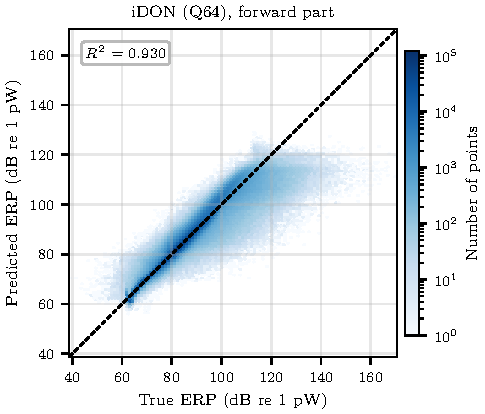
\includegraphics[max width=\textwidth]{Bilder/idon_forward_prediction_vs_true_erp.pdf}
\caption[iDON forward predicted versus true ERP]{iDON (Q64, forward direction): predicted ERP against the solver's ERP, across the full test split of the 200{,}000-configuration dataset.}
\label{fig:idon-forward-parity}
\end{figure}

Figure~\ref{fig:invertible-best} and Figure~\ref{fig:invertible-worst} show the best and the worst test spectrum of each invertible model in the forward direction. In the best cases all models follow the solver closely (RMSE 0.6 to 1.1\,dB, 1.9\,dB for iDON (Q8)). In the worst cases the errors are 6.0\,dB for iDON (Q64), 6.7 to 9.3\,dB for the family and 13.7\,dB for iDON (Q8); the largest deviations occur where the solver curve has several narrow, closely spaced peaks, as for the forward architectures, and in several of them a resonator sits right next to the force position.

\begin{figure}[p]
\centering
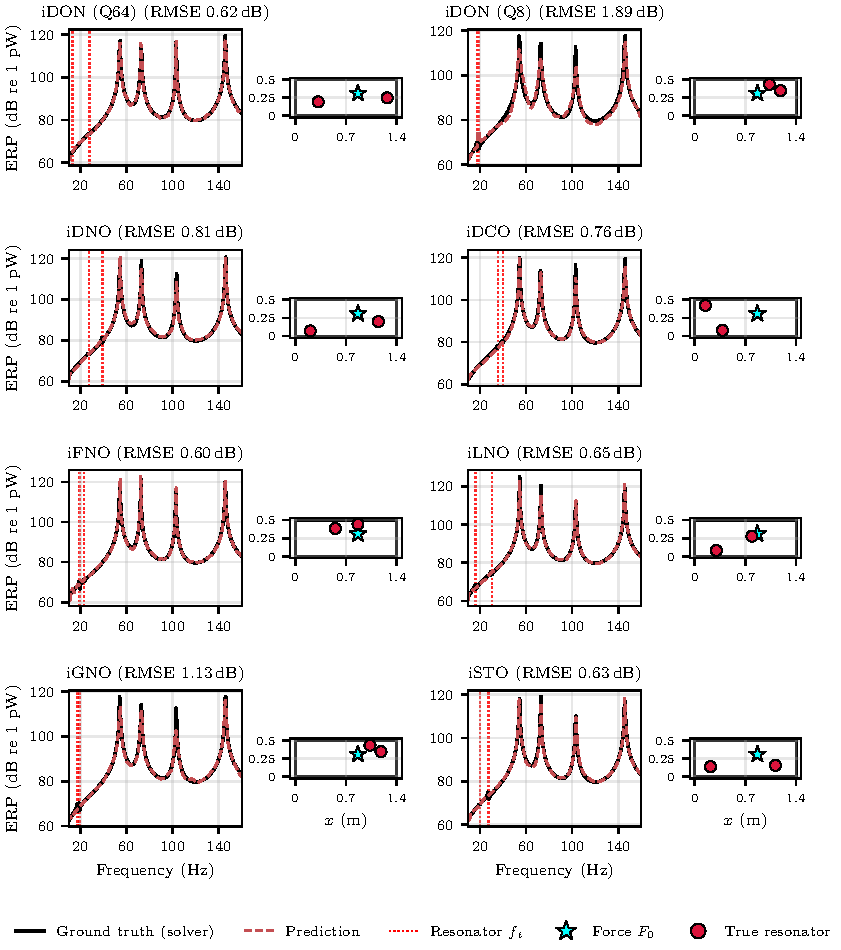
\includegraphics[max width=\textwidth,max height=0.84\textheight]{Bilder/invertible_models_forward_best_case.pdf}
\caption[Best forward prediction of each invertible model]{Forward direction of the invertible models on the 200{,}000-configuration dataset: for each model, the test spectrum with the lowest RMSE.}
\label{fig:invertible-best}
\end{figure}

\begin{figure}[p]
\centering
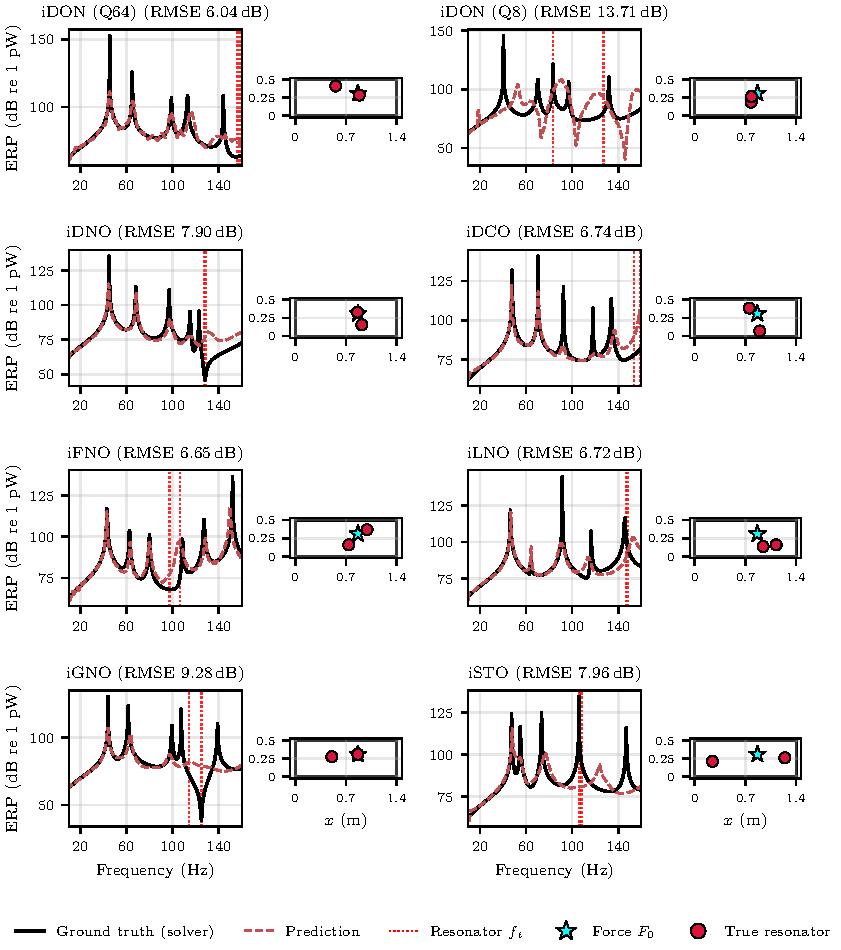
\includegraphics[max width=\textwidth,max height=0.84\textheight]{Bilder/invertible_models_forward_worst_case.pdf}
\caption[Worst forward prediction of each invertible model]{Forward direction of the invertible models on the 200{,}000-configuration dataset: for each model, the test spectrum with the highest RMSE.}
\label{fig:invertible-worst}
\end{figure}

Second, the inverse accuracy is far behind the forward accuracy for every model: around 7.8 to 8.1\,dB for the family instead of 2.4 to 3.8\,dB, and 5.8\,dB for iDON (Q64), the best inverse model, which is also the largest. The tuning frequency is recovered much better ($r(f_t)$ between 0.87 and 0.92) than the $y$ position ($r(y)$ between 0.12 for iDCO and 0.26 for iDNO). This matches the non-uniqueness argument made in Chapter~\ref{ch:theory}: many different resonator positions can produce a very similar spectrum, especially along the plate's short, 0.5\,m $y$ direction, so recovering a spectrum's tuning frequencies is a much better-posed problem than recovering exact positions. Figure~\ref{fig:ifno-inverse-example} shows the same target spectrum and the proposal selected by each model's own forward direction, together with the true and the proposed resonator positions on the plate. Every model reproduces the general rising shape of the spectrum and lines up with the target at several resonance peaks, but every model also proposes extra peaks the target does not have and misses others: iDON (Q64) matches almost all peaks (3.9\,dB), apart from one spurious peak near 33\,Hz, the family members reach 6.1 to 9.1\,dB, and iDON (Q8) fails to reproduce the spectrum (12.3\,dB). The plate in the lower panel shows why the proposals differ from the truth: most proposed resonators lie in the neighbourhood of the force and of the first true resonator, none of them is placed near the second true resonator at the lower plate edge, and almost all proposed positions lie between $y = 0.2$ and $0.35$\,m, around the centre line of the plate.

\begin{figure}[p]
\centering
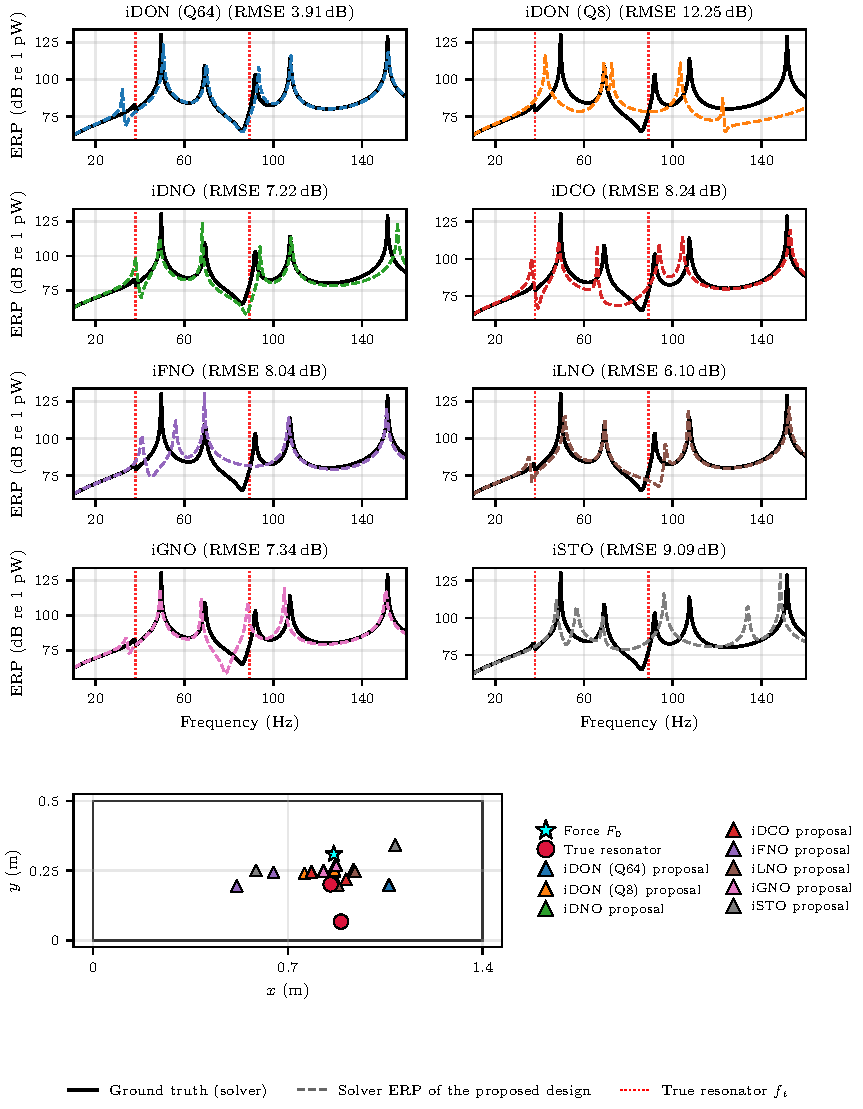
\includegraphics[max width=\textwidth,max height=0.84\textheight]{Bilder/invertible_models_inverse_prediction.pdf}
\caption[Inverse design example, all invertible models]{One target spectrum (black) and the proposal selected by the own forward direction (coloured, 8 samples per model) from all invertible models, re-simulated with the solver. The plate shows the two true resonators (red circles) and the proposed resonators of every model (triangles in the colour of the model).}
\label{fig:ifno-inverse-example}
\end{figure}

Figure~\ref{fig:idon-inverse-parameters} shows the same weakness over many targets, for iDON (Q64): for 4{,}000 test targets, the proposed value of each design variable against the true one. The tuning frequency lies on the diagonal ($r = 0.87$) and the $x$ position follows it clearly ($r = 0.69$), whereas the mass is only loosely recovered ($r = 0.40$) and the $y$ position collapses onto a narrow band around $y \approx 0.25$\,m ($r = 0.29$): the model proposes a $y$ position near the plate's centre line almost regardless of the target, presumably because the spectrum constrains it only weakly.

\begin{figure}[h]
\centering
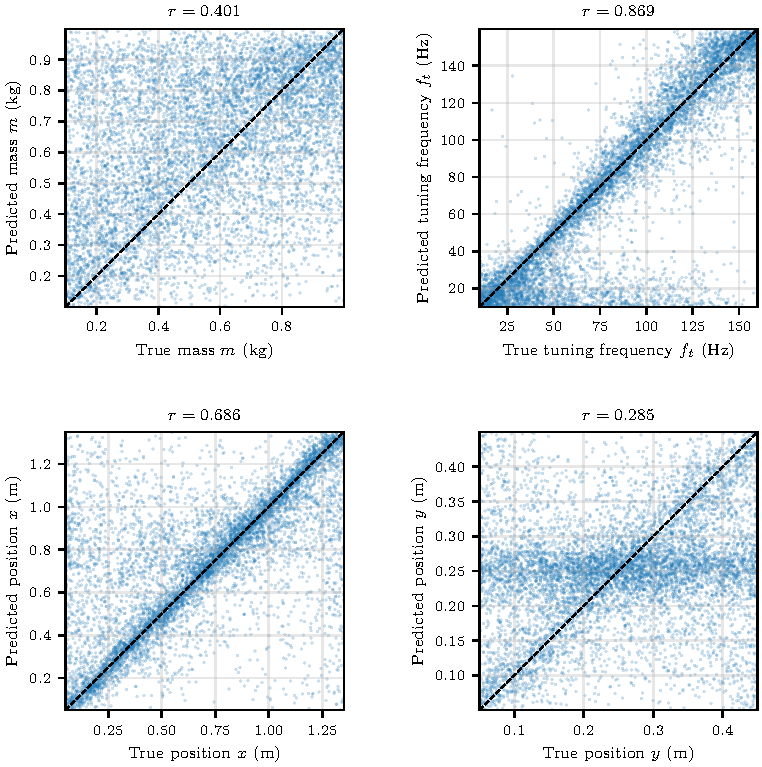
\includegraphics[max width=\textwidth]{Bilder/idon_inverse_prediction_vs_true_parameters.pdf}
\caption[iDON: predicted versus true resonator parameters]{iDON (Q64, inverse direction): proposed against true resonator parameters for 4{,}000 test targets (one sample per target, selected by the model's own forward direction; resonators ordered by tuning frequency).}
\label{fig:idon-inverse-parameters}
\end{figure}

Third, iDON is evaluated separately, since its design-size parameter $Q$ is itself a modelling choice, discussed in Section~\ref{sec:idon}. Table~\ref{tab:idon-q} confirms the effect of padding beyond the design size $D=8$ numerically: Q64 is clearly better than Q8 on every metric, including the position-recovery error, which is reported directly in centimetres rather than as a correlation, and which is roughly halved. One caveat applies to this comparison: the Q8 training run stopped early, after 50 of the 150 planned epochs (Section~\ref{sec:training}), so part of its disadvantage may come from the shorter training and not from the missing padding alone.

\begin{table}[h]
\centering
\caption[iDON: Q8 versus Q64]{iDON with the design-sized basis (Q8, $Q=D=8$) against the padded basis (Q64, $Q=64$): inverse results for 500 test targets, 16 samples each (selected by the own forward direction); the forward RMSE is that of the full test split.}
\label{tab:idon-q}
\begin{tabular}{lrrrr}
\hline
Variant & Fwd RMSE (dB) & Inv RMSE (dB) & $r(f_t)$ & Median position error (cm) \\
\hline
Q8  & 6.047 & 9.969 & 0.812 & 24.4 \\
Q64 & 2.673 & 5.165 & 0.867 & 12.8 \\
\hline
\end{tabular}
\end{table}

Taken together, these results show that the forward half of every invertible architecture works reasonably well, although less accurately than a dedicated forward architecture, and that the inverse direction already recovers the overall shape of a target spectrum and its dominant tuning frequencies reasonably well, while exact position recovery remains the hardest part of generative design with this approach, a limitation discussed further in Chapter~\ref{ch:conclusions}.

\FloatBarrier
\newpage
\chapter{Conclusions and Outlook}
\label{ch:conclusions}
This thesis set out to work toward generative design of tuned mass resonator layouts on a plate: given a target equivalent radiated power spectrum, propose a resonator design that achieves it. To reach that goal, a design space of five variables per resonator, mass, tuning frequency, position and a damping ratio, was defined and sampled evenly with Latin hypercube sampling, and datasets of 100{,}000 two-resonator and 100{,}000 three-resonator configurations were generated with a modal physics solver. Ten forward neural network architectures were then built and compared as fast surrogates for that solver, and seven invertible architectures were developed and evaluated that predict a spectrum from a design and propose a design from a spectrum with a single set of weights.

The forward comparison showed that an explicit, permutation-invariant resonator encoder combined with physics-aware frequency features matters: every architecture that uses them clearly outperforms the plain feed-forward baseline, and the best architecture, DCO, reaches about 1.1\,dB root-mean-square error against the solver on unseen two-resonator designs. The top and the bottom of the ranking held on a three-resonator dataset, where the error of the architectures increased by a factor of 1.1 to 2.0 (DCO from 1.1\,dB to 2.2\,dB), confirming that the comparison reflects a real property of each architecture rather than an artefact of the simpler two-resonator case. A separate experiment, reported in Appendix~A, showed that these forward models interpolate well within the frequency band they are trained on but lose accuracy once asked to extrapolate beyond it, which is a useful caution for how the surrogates should be used.

In the forward direction the invertible architectures reached 2.4 to 3.8\,dB RMSE (2.7\,dB for iDON), which is comparable to the plain forward architectures on the harder three-resonator dataset but behind them on the two-resonator dataset (1.1 to 2.1\,dB for eight of the ten); since the datasets differ, this comparison is only indicative, but it suggests that making a core invertible costs some forward accuracy. Their inverse direction already recovers the overall shape of a target spectrum and its dominant tuning frequencies reasonably well, with correlations around 0.9 for the tuning frequency. Recovering exact resonator positions is markedly harder, with correlations as low as 0.12 for some architectures, because many different layouts can produce a nearly identical spectrum, as the non-uniqueness example in Chapter~\ref{ch:theory} showed directly. For iDON, padding the invertible branch beyond the design's own size made a clear difference on every metric checked, including halving the median position-recovery error, which shows that the capacity of the invertible core, not just its architecture, matters for how well the inverse direction performs.

These invertible results come from an earlier, four-variable version of the design space, built before the damping ratio and before the final two-resonator, 100{,}000-configuration forward dataset used in Chapter~\ref{ch:results}. Retraining the invertible architectures on the current five-variable design space is therefore the most direct next step: it is what would turn the forward surrogates and invertible architectures built in this thesis into one consistent generative design tool. Beyond that, four further steps follow from the results in this thesis. First, improving position recovery specifically, for example by giving the inverse direction an explicit way to represent several equally valid proposals rather than averaging over them, as the probabilistic inverse models of \textcite{thorpe2025generalizable} or the generative latent-space formulation of \textcite{zang2026designgenno} do. Second, extending the invertible models from two resonators to three, the way the forward comparison was already extended in Chapter~\ref{ch:results}. Third, applying the Monte Carlo uncertainty quantification procedure described in Chapter~\ref{ch:theory} to proposed designs, to check that a design the invertible operator suggests still meets its target once small, realistic manufacturing tolerances are taken into account. Fourth, validating a proposed design experimentally on a real plate, to check that the gap between the solver and reality does not undo what the neural operators learned from simulation alone.

Taken together, this thesis provides forward surrogates for two and three resonators, invertible architectures that already perform generative design with reasonable spectrum and tuning-frequency accuracy, and a reproducible, single-script pipeline for all of it, while identifying position recovery and retraining on the current design space as the concrete next steps toward a complete generative design tool.

\FloatBarrier
\newpage
\medskip
\printbibliography

\addcontentsline{toc}{chapter}{Bibliography}
\newpage
\appendix
\chapter{Frequency Holdout: Extrapolation Beyond the Training Band}
The forward models in Chapter~\ref{ch:results} are trained and tested on frequencies drawn from the same 10 to 160\,Hz band, so a good test-split score only shows that a model can interpolate between frequencies it has already seen. A separate, smaller experiment checks a stricter question: can a model also handle a band of frequencies it never saw at all during training? This is kept out of the main results because it uses an earlier, 3-resonator dataset of 10{,}000 configurations rather than the 2-resonator, 5-variable dataset used everywhere else in this thesis, and because it only answers a secondary question about extrapolation, not the generative-design objective of the thesis.

\section{Setup}

The middle 20\,\% of the frequency band, 70 to 100\,Hz, is removed completely from training and validation: the models never see a solver spectrum value inside this band while learning. After training, each model is evaluated on the full band and scored separately on the frequencies it trained on (``seen'') and the held-out band (``unseen''). A large gap between the two scores means a model has mostly memorised input-output pairs at the frequencies it was shown, rather than learning the underlying physics well enough to fill in a gap.

Six of the ten architectures from Chapter~\ref{ch:results} are included in this experiment: DON, DNO, DCO, WNO, GNO and NN.

\section{Results}

\begin{table}[h]
\centering
\caption[Seen vs. unseen RMSE in the frequency-holdout experiment]{Root-mean-square error (RMSE), mean absolute error (MAE) and Pearson correlation on the seen frequencies versus the held-out 70--100\,Hz band.}
\begin{tabular}{lrrrrrr}
\hline
Model & RMSE seen & RMSE unseen & MAE seen & MAE unseen & $r$ seen & $r$ unseen \\
\hline
DNO & 3.98 & 7.11 & 1.95 & 4.45 & 0.922 & 0.544 \\
DCO & 3.95 & 7.38 & 1.94 & 4.83 & 0.924 & 0.521 \\
NN  & 4.88 & 7.17 & 2.86 & 4.72 & 0.880 & 0.493 \\
GNO & 4.10 & 7.67 & 2.11 & 4.99 & 0.917 & 0.439 \\
WNO & 5.59 & 8.92 & 3.07 & 6.39 & 0.840 & 0.258 \\
DON & 6.35 & 13.37 & 3.93 & 10.31 & 0.812 & 0.125 \\
\hline
\end{tabular}
\end{table}

Every model is clearly worse on the held-out band: RMSE roughly doubles to triples, and the Pearson correlation on the unseen band drops well below the seen-band value for every architecture. DNO and DCO cope best with the gap, while DON is affected the most. Figure~\ref{fig:holdout-example} shows one example spectrum from this experiment: the solver curve and the model prediction agree closely outside the grey band, but the model prediction departs from the solver curve inside it.

\begin{figure}[h]
\centering
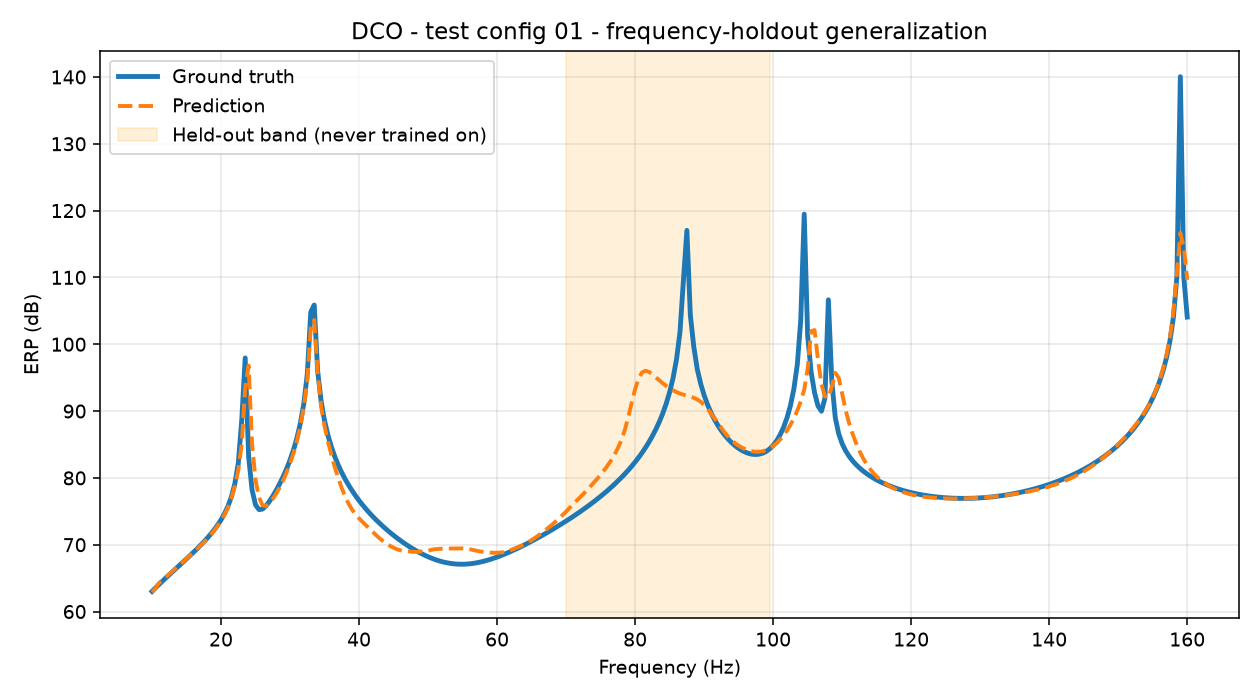
\includegraphics[width=0.85\textwidth]{Bilder/holdout_example.png}
\caption[Example spectrum from the frequency-holdout experiment]{Example test spectrum from the frequency-holdout experiment. The model was never trained on the shaded 70--100\,Hz band.}
\label{fig:holdout-example}
\end{figure}

The practical conclusion is simple: these forward surrogates are reliable for interpolating within the frequency band they were trained on, which is exactly how they are used in this thesis, but they should not be trusted to extrapolate to frequencies outside their training range without retraining on data that covers that range.

\newpage
\chapter{Attachment}
The code and data this thesis is grounded in are available at the following locations:
\begin{itemize}
  \item \textbf{GitHub:} \url{https://github.com/sherirashmi/master_thesis_2026}
  \item \textbf{LRZ Sync\&Share:} \url{https://syncandshare.lrz.de/getlink/fi7b5Si4RZ3p21L3YKyupu/}
\end{itemize}
Contents:
\begin{itemize}
  \item \texttt{erp\_neural\_operators.py}: solver, dataset generation, forward and invertible models
  \item the datasets and the trained models
\end{itemize}
Updates, in particular retrained invertible operators (see Section~\ref{sec:training}), will be published in the GitHub repository.

\newpage
\thispagestyle{empty}
\section*{Erklärung}

Ich versichere hiermit, dass ich die von mir eingereichte Abschlussarbeit selbstständig verfasst und keine anderen als die angegebenen Quellen und Hilfsmittel benutzt habe. Bei der Erstellung dieser Arbeit habe ich die Unterstützung des KI-Assistenten Claude (Anthropic) in Anspruch genommen.

\vspace*{50pt}


\hrule
\vspace*{5pt}
Ort, Datum, Unterschrift

\vspace*{140pt}


\end{document} 